\documentclass[a4paper,11pt]{article}
\usepackage[brazilian]{babel}
\usepackage[utf8]{inputenc}
\usepackage[T1]{fontenc}
\usepackage{epsfig}
\usepackage{array}


\usepackage{scrextend}

\usepackage{graphicx, url}
\usepackage[usenames]{color}
\usepackage{rotating}
\usepackage{url}
\usepackage{pdfpages}
\usepackage{subfigure}
\usepackage[table]{xcolor}
\usepackage{xspace}
\usepackage[verbose, dvips=true, pdftex=false, vtex=false, paperwidth=210mm,paperheight=295mm,top=35mm,left=30mm,bottom=35mm,right=30mm]{geometry}
\usepackage[authoryear]{natbib}
\usepackage{fancyhdr}
\usepackage{setspace}


\DeclareGraphicsExtensions{.png,.jpg,.pdf,.mps}
\bibliographystyle{icmc2}

\clubpenalty=10000
\widowpenalty=10000
\newcommand{\rev}[1]{{\color{red}#1}}

\newcommand{\titlehd}{\sffamily\bfseries\selectfont \scriptsize Uma Abordagem de Reestruturação de Sistemas Baseada em Requisitos de Qualidade Pré-Estabelecidos }

\pagestyle{fancy}
\headheight 61pt
\fancyhead{}
\fancyhead[LO]{
\epsfig{file=icmc.jpg,height=15mm}}
\fancyhead[RO]{}
\fancyfoot{}

\begin{document}

\begin{center}
\vspace*{1cm}
{\fontsize{17.28}{20}\sffamily\bfseries\selectfont Uma Abordagem de Reestruturação de Sistemas Baseada em Requisitos de Qualidade Pré-Estabelecidos \\\ \\

\small{RELATÓRIO CIENTÍFICO PARCIAL - 01/06/2012 a 15/03/2013}\\ \
\textsf{Apresentado à Fundação de Amparo à Pesquisa do Estado de São Paulo - FAPESP}
 \\
\vspace{3cm}}


\begin{table}[!th]
  \begin{center}
    \begin{tabular}{ll}

	  Número do Processo:      &   FAPESP 2012/05168-4     \\
      Período:        &  Junho/2012 a Março/2013                    \\
	                   &                                \\
      Bolsista:           &  Rafael Serapilha Durelli (rdurelli@icmc.usp.br)                                     \\
	  
	  \vspace{0.6cm}
      Orientador:        &  Prof. Dr. Márcio E. Delamaro (delamaro@icmc.usp.br)                                           \\

	         &                              \\
	          &  \\
                       &                                  \\
       &                                       \\
              &                                             \\ \\
      \vspace{1cm}

    \end{tabular}
  \end{center}
\end{table}

\vfill
{\fontsize{18}{20}\sffamily\bfseries\selectfont USP - São Carlos \\ Janeiro de 2012}

\end{center}

\vspace{3cm}

\pagebreak
\fancyhead[RO]{\titlehd}
\fancyfoot{\centerline{\thepage}}
\setcounter{page}{1}

\parskip 6pt

\doublespacing
\begin{abstract}
 Relatório Científico Parcial apresentado à FAPESP (Fundação de Amparo à Pesquisa do Estado de São Paulo) com o objetivo de elucidar as atividades realizadas  
 pelo bolsista Rafael Serapilha Durelli durante o primeiro período de vigência da bolsa concebida sob o Processo Número 2012/05168-4. 
 O referido período teve inicio em Junho de 2012 e foi finalizado em Março de 2013. 
 Além disso, este relatório também descreve as atividades que estão em andamentos, bem como as atividades a serem realizadas no próximo período. 
 Vale ressaltar que a partir de resultados preliminares alguns artigos científicos foram elaborados e publicados.
%Software é um produto que tende a evoluir constantemente com o intuito de satisfazer às necessidades de seus usuários. Para isso é necessário submetê-lo a constantes atividades de manutenção, que podem ocasionar um possível degradação no código-fonte. Dessa forma, o objetivo desta proposta de doutorado é o desenvolvimento de uma abordagem que auxilie o engenheiro de software a escolher o melhor conjunto de transformações para um sistema legado com base em requisitos de qualidade pré-estabelecidos e com isso possa identificar o impacto que tais transformações irão ocasionar no sistema legado. Isto é, a abordagem deverá indicar conjuntos de possíveis transformações para a evolução do sistema legado, além disso, deverá informar ao engenheiro o quanto tais transformações irão afetar a evolução/estrutura desse sistema. Com isso, o engenheiro de software poderia previamente escolher qual o melhor conjunto de  transformação se aplica dado um requisito de qualidade pré-estabelecido. Após a escolha das transformações a abordagem também deverá realizar automaticamente tais transformações a fim de reestruturar o sistema legado em um novo sistema. Será avaliado a abordagem por meio de experimentos controlados.

\end{abstract}


      



\section{Introdução}
	 Este relatório tem por objetivo apresentar as atividades realizadas pelo bolsista Rafael Serapilha Durelli durante o período de Junho/2012 a Março/2013,
 referente à bolsa de doutorado concebida pela Fundação de Amparo à Pesquisa do Estado de São Paulo (FAPESP) sob o Processo Número 2012/05168-4. 
 
 É importante salientar que o trabalho em questão tem sido desenvolvido no Departamento de Ciências da Computação e Estatística do Instituto de Ciência 
 Matemáticas e de Computação (ICMC) da Universidade de São Paulo (campos São Carlos/SP).  
 Este trabalho se insere no contexto do grupo de pesquisas em Engenheira de Software, sob a orientação do Prof. Dr. Márcio Eduardo Delamaro.  
 Além disso, este trabalho esta sendo executado em colaboração com o grupo de engenharia de software da Universidade Federal de São Carlos (UFSCAR)\footnote{http://dc.ufscar.br}.  
 Mais especificamente em colaboração com o Prof. Dr. Valter Vieira de Camargo\footnote{http://buscatextual.cnpq.br/buscatextual/visualizacv.do?id=S819089},
 o qual tem grande experiência na área de engenharia de software com ênfase no desenvolvimento de frameworks no contexto da programação orientada a aspectos e reuso de software. 

Por fim, ressalta-se que o bolsista criou um vínculo científico com o \textit{Institut National de Recherche en Informatique et en Automatique} (INRIA),  
onde irá realizar um ano de doutorado sanduíche sobre orientação do  
 Prof. Dr. Nicolas Anquetil\footnote{http://rmod.lille.inria.fr/web/pier/team/Nicolas-Anquetil} o qual tem grande experiência na área de manutenção e reengenharia de software.

\section{Plano de Trabalho}\label{plano_trabalho}
	Nesta seção são apresentados os resumos tando do plano de trabalho quanto das atividades conduzidas durante esse primeiro período de vigência da bolsa. Adicionalmente, apresenta-se o cronograma inicialmente proposto.

		
		\subsection{Resumo do Plano Inicial}\label{resumo_plano_inicial}
			
Muitas organizações utilizam sistemas que foram desenvolvidos há anos e que já foram submetidos a diversas atividades de manutenção para se adequar a novos requisitos, acomodar alterações tecnológicas e satisfazer novos processos de negócio. Sistemas que não foram projetados de forma adequada para acomodar constantes alterações em seus requisitos, tendem a ter suas arquiteturas corrompidas e rapidamente tornam-se obsoletos, trazendo dificuldades para o crescimento da organização em ambientes competitivos. Quando isso ocorre, esses sistemas são comumente conhecidos como ``sistemas legados''~\cite{Griffith2011}. 

De acordo com~\citet{Fokaefs2012} a partir do momento em que um sistema começa a ser utilizado, ele entra em um estado contínuo de mudança. Tais sistemas tendem a se tornarem obsoletos em vista das novas tecnologias que são disponibilizadas ou em consequência de manutenções que são feitas sem planejamento. Além das correções de erros, as mudanças mais comuns que os sistemas sofrem são migrações para novos paradigmas e extensões em sua funcionalidade para atender a novos requisitos dos usuários. 

Os problemas mais comuns de sistemas legados são: (\textit{i}) tipicamente são implementados com tecnologias obsoletas fazendo com que a manutenção se torne custosa e difícil, (\textit{ii}) usualmente não possuem documentações, e quando possuem, não estão atualizadas e (\textit{iii}) devido a falta de documentação, integrar sistemas legados à outros sistemas tende a ser um processo difícil, lento e propício a erros. No entanto, sistemas legados tem geralmente uma missão importante dentro de uma companhia pois representam/armazenam informações de suma importância e assim não podem simplesmente serem descartados.


Outro problema é que muitas tarefas de manutenção necessitam de grandes modificação no código-fonte, as quais são normalmente feitas manualmente e assim tendem a gerarem efeitos colaterais em outros módulos do sistema. Além disso, em geral, processos de manutenção são iniciados sem uma clara especificação do que se quer alcançar, dificultando a identificação se o problema foi resolvido completamente.



Uma das técnicas disponíveis na literatura para melhorar a qualidade de sistemas legados é submetê-los a um processo de reengenharia que é o processo no qual ``transformações'' são realizadas no sistema com o intuito de melhorar sua estrutura sem alterar seu comportamento original~\cite{refactImpro}.  



Usualmente reengenharia está ligada com transformações as quais seguem catálogos de refatorações, tais como as refatorações propostas por~\citet{refactImpro}. Transformação é a atividade em que um conjunto de mudanças são efetivamente realizadas no código-fonte, objetivando melhorar sua estrutura e até mesmo atender a novos requisitos~\cite{Griswold}. Para auxiliar essa atividade algumas abordagens existem na literatura~\cite{bisbal, tilley, refactImpro}.

Similarmente várias abordagens foram propostas para auxiliar a reengenharia de sistemas legados~\cite{Griffith2011, Olszak:2012:RJP:2108329.2108539}.
Apesar da existência de todas essas abordagens, de acordo com~\citet{Sneed:2005} mais da metade dos projetos que aplicam reengenharia falham ao lidar com desafios específicos. Segundo tal autor, tanto a carência de  padronização durante a atividade de reengenharia quanto a falta de apoio computacional efetivo são os principais problemas que acarretam esse grande número de falhas.  A falta de um processo padronizado é um problema durante a atividade de reengenharia, a qual é realizada de maneira totalmente \textit{ad hoc}. Adicionalmente, o código-fonte não deve ser o único artefato do software a possuir padronização, uma vez que o mesmo não representa/contêm todas as informações necessárias de um sistema. Portanto, a atividade de reengenharia deve possuir diretrizes que auxiliem a padronização de todos os artefatos do software, e.g., código-fonte, dados, regras de negócios, etc.


Uma alternativa à reengenharia tradicional e que vem sendo investigada atualmente é a Modernização Orientada à Arquitetura (\textit{Architecture Driven Modernization} - (ADM)), a qual permite realizar análises de descoberta de conhecimento e refatorações utilizando os princípios da abordagem de Desenvolvimento Orientado a Modelos (\textit{Model-Driven Development} - (MDD)), ao invés de efetuá-los diretamente no código-fonte~\cite{PerezCastillo:2011jo}. 

Uma forte característica da ADM é o oferecimento de um conjunto de metamodelos padronizados para representar artefatos de um sistema legado. Entre esses metamodelos tem-se o principal ativo da OMG, denominado metamodelo de Descoberta de Conhecimento (\textit{Knowledge Discovery Meta-Model} - KDM). KDM é um metamodelo para instanciar e modelar todos os artefatos de um sistema legado e pode ser utilizado como um metamodelo independente para auxiliar o engenheiro de software durante a atividade de modernização de sistemas legados. Entre Maio de 2004 e Agosto de 2005, mais de trinta organizações colaboraram para o desenvolvimento e revisão da padronização do KDM. Em meados de 2007, a OMG oficializou a versão 1.0 do KDM, e hoje o KDM encontrasse na versão 1.3 e é reconhecido internacionalmente como uma padronização (ISO/IEC 19506) para ser utilizado durante a atividade de modernização de sistemas legados~\cite{ISOKDM}. 


Este projeto de doutorado tem quatro principais motivações. A primeira é a carência de catálogos de refatorações para o metamodelo KDM. Existem documentos~\cite{OMGADM, ADMBook, ADMCHAPTERR} que mostram que refatorações para esse metamodelo ainda não existem. Neste contexto, é importante criar catálogos de refatorações para o KDM com objetivo de padronizar o processo de modernização e aumentar a interoperabilidade entre ferramentas que utilizam o KDM para auxiliar o processo de modernização.


A segunda motivação é a ausência de abordagens que permitam analisar diferentes cenários de modernização antes de efetivamente realizar transformações no sistema legado. A maior parte das abordagens disponíveis na literatura realizam as refatorações diretamente no código-fonte. Assim, tais abordagens inviabilizam a possibilidade de gerar vários sistemas modernizados somente para averiguar qual deles é o mais adequado de acordo com os modelos de referência. No contexto deste projeto, modelos de referência são especificações do que se espera que o sistema legado atenda após ser modernizado, por exemplo, uma arquitetura orientada a serviço.


A terceira motivação é a falta de meios para se especificar tais modelos de referência. Portanto, muitas tarefas de reengenharia são iniciadas sem um entendimento claro dos problemas atuais e sem uma definição precisa das melhorias esperadas após as refatorações; fazendo com que não sejam efetivas na solução dos problemas existentes. O que as abordagens de refatoração atuais fazem é aplicar o mesmo conjunto de casos de teste nas duas versões do sistema e averiguar se a funcionalidade não foi alterada~\cite{Demeyer1, Demeyer2, RefactoringJava}. Entretanto, isso não garante que os problemas foram resolvidos.


Por fim, existe a necessidade de um apoio computacional efetivo durante a atividade de reengenharia de um sistema legado. Como ressaltado anteriormente, mais da metade dos projetos que aplicaram reengenharia em um sistema legado falharam devido a ausência de um apoio computacional efetivo~\cite{Sneed:2005}. A falta de padronização durante a atividade de reengenharia também acarreta esse grande número de falhas. Sem uma padronização a atividade de reengenharia tente a ser realizada de maneira totalmente \textit{ad hoc}, o que pode atrasar e gerar gastos durante a atividade em questão.


Tendo elucidado os problemas relacionados com a reengenharia de software, o objetivo deste projeto é desenvolver um ambiente que recomende cenários alternativos de modernização com base em modelos de referência. Adicionalmente, objetiva-se desenvolver catálogos de refatorações para o metamodelo KDM. Com a utilização desses catálogos será possível fazer com o que sistemas legados sejam refatorados para uma arquitetura orientada a serviços ou outras arquiteturas candidatas. Do mesmo modo será possível que interesses transversais de um sistema legado sejam refatorados para se tornarem mais modular, por exemplo, utilizando o paradigma orientada a aspectos~\cite{Kiczales}. 


%Tendo elucidado os problemas relacionados com a reegenharia de software, o objetivo deste projeto é desenvolver um ambiente que recomende cenários alternativos de modernização com base em modelos de referência. Por exemplo, o ambiente deverá comparar o resultado da modernização com o que foi especificado no modelo de referência e indicar possíveis desvios de cada cenário. Uma vez que pretende-se permitir que o engenheiro de software manipule diferentes cenários de modernização do mesmo sistema legado simultaneamente, uma possível abordagem é alterar diversas vezes o menos código-fonte do sistema. No entanto, essa abordagem tende a consumir grande quantidade de recurso computacional~\cite{Lavallee2011}. Outra possível abordagem, e é a que será utilizada neste projeto é a utilização de modelos mais abstratos do que o código-fonte. Portanto, cada cenário de modernização será representado por pelo metamodelo KDM para auxiliar na representação dos artefatos do sistema legado.



 



		\subsection{Cronograma}\label{cronograma}
			A seguir é apresentado o cronograma que esta sendo seguido pelo bolsista para o desenvolvimento deste projeto. Em seguida, é apresentada uma descrição de cada atividade presente no cronograma.

\begin{table}[!h]
\centering
\caption{Cronograma de Atividades}



{\tiny }%
\begin{tabular}{|c|>{\centering}p{1bp}|>{\centering}p{1bp}|>{\centering}p{1bp}|>{\centering}p{1bp}|>{\centering}p{1bp}|>{\centering}p{1bp}|>{\centering}p{1bp}|>{\centering}p{1bp}|>{\centering}p{1bp}|>{\centering}p{1bp}|>{\centering}p{1bp}|>{\centering}p{1bp}|>{\centering}p{1bp}|>{\centering}p{1bp}|>{\centering}p{1bp}|>{\centering}p{1bp}|>{\centering}p{1bp}|>{\centering}p{1bp}|>{\centering}p{1bp}|>{\centering}p{1bp}|>{\centering}p{1bp}|>{\centering}p{1bp}|>{\centering}p{1bp}|>{\centering}p{1bp}|>{\centering}p{1bp}|>{\centering}p{1bp}|>{\centering}p{1bp}|>{\centering}p{1bp}|>{\centering}p{1bp}|}
\cline{2-30} 
\multicolumn{1}{c|}{} & \multicolumn{3}{c|}{\textbf{\tiny 2011}} & \multicolumn{6}{c|}{\textbf{\tiny 2012}} & \multicolumn{6}{c|}{\textbf{\tiny 2013}} & \multicolumn{6}{c|}{\textbf{\tiny 2014}} & \multicolumn{6}{c|}{\textbf{\tiny 2015}} & \multicolumn{2}{c|}{\textbf{\tiny 2016}}\tabularnewline
\cline{2-30} 
\multicolumn{1}{r|}{\begin{sideways}
\textbf{\tiny ATIVIDADES}
\end{sideways}} & \begin{sideways}
\textbf{\tiny Jul-}{\tiny \par}

\textbf{\tiny Ago}
\end{sideways} & \begin{sideways}
\textbf{\tiny Set-Out}
\end{sideways} & \begin{sideways}
\textbf{\tiny Nov-Dez}
\end{sideways} & \begin{sideways}
\textbf{\tiny Jan-}{\tiny \par}

\textbf{\tiny Fev}
\end{sideways} & \begin{sideways}
\textbf{\tiny Marc-Abr}
\end{sideways} & \begin{sideways}
\textbf{\tiny Mai-Jun}
\end{sideways} & \begin{sideways}
\textbf{\tiny Jul-Ago}
\end{sideways} & \begin{sideways}
\textbf{\tiny Set-Out}
\end{sideways} & \begin{sideways}
\textbf{\tiny Nov-Dez}
\end{sideways} & \begin{sideways}
\textbf{\tiny Jan-Fev}
\end{sideways} & \begin{sideways}
\textbf{\tiny Marc-Abr}
\end{sideways} & \begin{sideways}
\textbf{\tiny Mai-Jun}
\end{sideways} & \begin{sideways}
\textbf{\tiny Jul-Ago}
\end{sideways} & \begin{sideways}
\textbf{\tiny Set-Out}
\end{sideways} & \begin{sideways}
\textbf{\tiny Nov-Dez}
\end{sideways} & \begin{sideways}
\textbf{\tiny Jan-Fev}
\end{sideways} & \begin{sideways}
\textbf{\tiny Marc-Abr}
\end{sideways} & \begin{sideways}
\textbf{\tiny Mai-Jun}
\end{sideways} & \begin{sideways}
\textbf{\tiny Jul-Ago}
\end{sideways} & \begin{sideways}
\textbf{\tiny Set-Out}
\end{sideways} & \begin{sideways}
\textbf{\tiny Nov-Dez}
\end{sideways} & \begin{sideways}
\textbf{\tiny Jan-Fev}
\end{sideways} & \begin{sideways}
\textbf{\tiny Marc-Abr}
\end{sideways} & \begin{sideways}
\textbf{\tiny Mai-Jun}
\end{sideways} & \begin{sideways}
\textbf{\tiny Jul-Ago}
\end{sideways} & \begin{sideways}
\textbf{\tiny Set-Out}
\end{sideways} & \begin{sideways}
\textbf{\tiny Nov-Dez}
\end{sideways} & \begin{sideways}
\textbf{\tiny Jan-Fev}
\end{sideways} & \begin{sideways}
\textbf{\tiny Marc-Abr}
\end{sideways}\tabularnewline
\hline 
\textbf{\tiny 1} & \textcolor{black}{\tiny \cellcolor{black!25}X} & \textcolor{black}{\tiny \cellcolor{black!25}X} & \textcolor{black}{\tiny \cellcolor{black!25}X} & \textcolor{black}{\tiny \cellcolor{black!25}X} & \textcolor{black}{\tiny \cellcolor{black!25}X} & \textcolor{black}{\tiny \cellcolor{black!25}X} & \textcolor{black}{\tiny \cellcolor{black!25}X} &  &  &  &  &  &  &  &  &  &  &  &  &  &  &  &  &  &  &  &  &  & \tabularnewline
\hline 
\textbf{\tiny 2} & \textcolor{black}{\tiny \cellcolor{black!25}X} & \textcolor{black}{\tiny \cellcolor{black!25}X} & \textcolor{black}{\tiny \cellcolor{black!25}X} & \textcolor{black}{\tiny \cellcolor{black!25}X} & \textcolor{black}{\tiny \cellcolor{black!25}X} & \textcolor{black}{\tiny \cellcolor{black!25}X} & \textcolor{black}{\tiny \cellcolor{black!25}X} & \textcolor{black}{\tiny \cellcolor{black!25}X} & \textcolor{black}{\tiny \cellcolor{black!25}X} &  &  &  &  &  &  &  &  &  &  &  &  &  &  &  &  &  &  &  & \tabularnewline
\hline 
\textbf{\tiny 3} &  &  &  &  &  & \textcolor{black}{\tiny \cellcolor{black!25}X} & \textcolor{black}{\tiny \cellcolor{black!25}X} & \textcolor{black}{\tiny \cellcolor{black!25}X} & \textcolor{black}{\tiny \cellcolor{black!25}X} &  &  &  &  &  &  &  &  &  &  &  &  &  &  &  &  &  &  &  & \tabularnewline
\hline 
\textbf{\tiny 4} &  &  &  &  &  &  &  &  &  & \textcolor{black}{\tiny \cellcolor{black!25}X} &  &  &  &  &  &  &  &  &  &  &  &  &  &  &  &  &  &  & \tabularnewline
\hline 
\textbf{\tiny 5} &  &  &  &  &  &  &  & \textcolor{black}{\tiny \cellcolor{black!25}X} &  &  &  &  &  &  &  &  &  &  &  &  &  &  &  &  &  &  &  &  & \tabularnewline
\hline 
\textbf{\tiny 6} &  &  &  &  &  &  &  & \textcolor{black}{\tiny X} & \textcolor{black}{\tiny X} & \textcolor{black}{\tiny X} & \textcolor{black}{\tiny X} & \textcolor{black}{\tiny X} & \textcolor{black}{\tiny X} & \textcolor{black}{\tiny X} &  &  &  &  &  &  &  &  &  &  &  &  &  &  & \tabularnewline
\hline 
\textbf{\tiny 7} &  &  &  &  &  &  &  &  & \textcolor{black}{\tiny X} & \textcolor{black}{\tiny X} & \textcolor{black}{\tiny X} & \textcolor{black}{\tiny X} & \textcolor{black}{\tiny X} & \textcolor{black}{\tiny X} & \textcolor{black}{\tiny X} & \textcolor{black}{\tiny X} &  &  &  &  &  &  &  &  &  &  &  &  & \tabularnewline
\hline 
\textbf{\tiny 8} &  &  &  &  &  &  &  &  &  &  &  &  & \textcolor{black}{\tiny X} & \textcolor{black}{\tiny X} & \textcolor{black}{\tiny X} & \textcolor{black}{\tiny X} & \textcolor{black}{\tiny X} & \textcolor{black}{\tiny X} &  &  &  &  &  &  &  &  &  &  & \tabularnewline
\hline 
\textbf{\tiny 9} &  &  &  &  &  &  &  &  &  & \textcolor{black}{\tiny X} & \textcolor{black}{\tiny X} & \textcolor{black}{\tiny X} & \textcolor{black}{\tiny X} & \textcolor{black}{\tiny X} & \textcolor{black}{\tiny X} & \textcolor{black}{\tiny X} &  &  &  &  &  &  &  &  &  &  &  &  & \tabularnewline
\hline 
\textbf{\tiny 10} &  &  &  &  &  &  &  &  &  &  &  &  &  &  & \textcolor{black}{\tiny X} & \textcolor{black}{\tiny X} & \textcolor{black}{\tiny X} & \textcolor{black}{\tiny X} & \textcolor{black}{\tiny X} & \textcolor{black}{\tiny X} &  &  &  &  &  &  &  &  & \tabularnewline
\hline 
\textbf{\tiny 11} &  &  &  &  &  &  &  &  &  &  &  &  &  &  &  &  & \textcolor{black}{\tiny X} & \textcolor{black}{\tiny X} & \textcolor{black}{\tiny X} & \textcolor{black}{\tiny X} &  &  &  &  &  &  &  &  & \tabularnewline
\hline 
\textbf{\tiny 12} &  &  &  &  &  &  &  &  &  &  &  &  &  & \textcolor{black}{\tiny X} &  & \textcolor{black}{\tiny X} &  & \textcolor{black}{\tiny X} &  & \textcolor{black}{\tiny X} &  &  & \textcolor{black}{\tiny X} & \textcolor{black}{\tiny X} & \textcolor{black}{\tiny X} & \textcolor{black}{\tiny X} & \textcolor{black}{\tiny X} & \textcolor{black}{\tiny X} & \tabularnewline
\hline 
\textbf{\tiny 13} &  &  &  &  &  &  &  &  &  &  &  &  &  &  &  &  &  &  &  &  &  & \textcolor{black}{\tiny X} & \textcolor{black}{\tiny X} & \textcolor{black}{\tiny X} & \textcolor{black}{\tiny X} & \textcolor{black}{\tiny X} & \textcolor{black}{\tiny X} & \textcolor{black}{\tiny X} & \tabularnewline
\hline 
\textbf{\tiny 14} &  &  &  &  &  &  &  &  &  &  &  &  &  &  &  &  &  &  &  &  &  &  &  & \textcolor{black}{\tiny X} & \textcolor{black}{\tiny X} & \textcolor{black}{\tiny X} & \textcolor{black}{\tiny X} &  & \tabularnewline
\hline 
\textbf{\tiny 15} &  &  &  &  &  &  &  &  &  &  &  &  &  &  &  &  &  &  &  &  &  &  &  &  &  &  &  &  & \textcolor{black}{\tiny X}\tabularnewline
\hline 
\end{tabular}
\end{table}

\begin{enumerate}
\item Realizar uma revisão sistemática para que o estado da arte referente ao tema de pesquisa relacionado a esta proposta de projeto seja obtido;
\item Obter créditos;
\item Escrever a monografia a ser apresentada no exame de qualificação;
\item Defender a qualificação;  
\item Realizar o exame de proficiência em língua estrangeira;
\item Investigar e combinar técnicas de mineração de interesses;
\item Estudar métricas para serem usadas durante a mineração de interesses;
\item Desenvolver um linguagem especifica de domínio e criar perfis do KDM para representar todos os artefatos de que um sistema legado possa possuir;
%\item Estudar métricas existentes na literatura que auxiliam a recomendar possíveis transformações para um determinado sistema legado;
%\item Estudar métricas existentes na literatura que auxiliam a classificar quantitativamente o impacto de um conjunto de transformações irá refletir no sistema legado;
\item Realização de 1 (um) ano de Dr. sanduíche em instituição estrangeira;
\item Elaborar algoritmos de recomendações de modernização para os sistemas legados;
\item Elaborar transformações que serão aplicadas nos sistemas legados e criar catálogos de refatorações para o KDM;
\item Escrever artigos científicos;
\item Elaborar e realizar experimentos para verificar a efetividade da abordagem desenvolvida;
\item Escrever a tese de doutorado;
\item Defender a tese de doutorado.  
\end{enumerate}

Ressalta-se que as atividades 7 à 10 do período Març-Abr/2013 à Març-Abr/2014 serão realizadas dentro de um programa de doutorado sanduíche.

\section{Resumo das Atividades Realizadas no Período}\label{atividades_realizadas}

	Nesta seção são apresentadas e detalhadas as atividades realizadas durante o primeiro período de bolsa,  
 correspondente aos meses de Junho/2012 a Março/2013.
 Em resumo, foram cursadas um conjunto de disciplinas para a obtenção dos créditos necessários do Programa de Pós-Graduação em Ciências de Computação e Matemática Computacional do ICMC. Além disso, estudou-se a abordagem Modernização Dirigida à Arquitetura
  ( em inglês - \textit{Architecture-Driven Modernization} - ADM), bem como seu principal ativo, o Meta-Modelo de Descoberta de Conhecimento (em inglês - \textit{Knowledge Discovery Meta-Model} - KDM). 

Realizou-se também uma revisão bibliográfica sistemática para investigar as principais técnicas e trabalhos disponíveis na literatura para auxiliar o desenvolvido do projeto em questão. O bolsista elaborou a monografia para o Exame de Qualificação e apresentou a mesma para a banca. Também são descritas nesta seção as publicações e eventos científicos nos quais o bolsista participou diretamente.

	\subsection{Atividades Técnicas Previstas no Cronograma do Projeto}

		\subsection{Disciplinas Regulares do Curso de Doutorado do ICMC/USP} % (fold)
\label{sub:disciplinas_regulares_do_curso_de_doutorado_do_icmc_usp}

De acordo com o tema central do projeto, foram escolhidas algumas disciplinas julgadas importantes para o bom aproveitamento do trabalho proposto no cronograma inicial. O quadro de disciplina cursadas pelo bolsista é mostrado a seguir:
% subsection disciplinas_regulares_do_curso_de_doutorado_do_icmc_usp (end)

\begin{enumerate}
	\item Engenharia de Software Experimental
		\begin{itemize}
			\item Carga Horária - 90
			\item Créditos: 6 (seis)
			\item Conceito Obtido: A
		\end{itemize}
	\item Revisão Sistemática em Engenharia de Software
		\begin{itemize}
			\item Carga Horária - 90
			\item Créditos: 6 (seis)
			\item Conceito Obtido: A
		\end{itemize}
	\item Validação e Teste de Software
		\begin{itemize}
			\item Carga Horária - 180
			\item Créditos: 12 (doze)
			\item Conceito Obtido: A
		\end{itemize}
	\item Preparação Pedagógica
		\begin{itemize}
			\item Carga Horária - 60
			\item Créditos: 4 (quatro)
			\item Conceito Obtido: A 
		\end{itemize}
	\item Especificação formal de software
		\begin{itemize}
			\item Carga Horária - 180
			\item Créditos: 12 (doze)
			\item Conceito Obtido: A
		\end{itemize}
\end{enumerate}

De acordo com as regras do Programa de Pós-Graduação em Ciências de Computação e Matemática Computacional do ICMC os alunos devem obter uma quantidade mínima de créditos para realizar determinadas tarefas, tais como, realizar o exame de qualificação e entregar a dissertação/tese. Nesse contexto, vale ressaltar que o bolsista em questão com o comprimento das disciplinas listadas a cima obteu-se um total de 40 créditos, sendo apto para realizar o exame de qualificação que exigi o mínimo de 24 créditos.%, bem como 36 créditos são necessários para o depósito da tese. 

Maiores informações sobre o desempenho do bolsista em cada uma das disciplinas e os conceitos obtidos podem ser avaliados mais cuidadosamente no histórico escolar deste relatório (ver Apêndice A).

%Conforme mencionado, durante o período deste relatório, o bolsista realizou tanto atividades técnicas requeridas para a concretização do seu projeto de doutorado quanto atividades exigidas pelo Programa de Pós-Graduação. Neste contexto, nesta subseção são apresentas e detalhadas as atividades técnicas realizadas até o momento. A seguir, cada uma das atividades realizadas é descrita.

\subsection{Estudo sobre Reengenharia de Software} % (fold)
\label{sub:reengenharia}


Software é um produto que evolui constantemente para satisfazer às necessidades de seus usuários. Para isso é necessário submetê-lo a constantes atividades de manutenção, que podem degradar o código-fonte, tornando-se cada vez mais difícil de mantê-lo uma vez que, na maioria das vezes, o software não é atulizado, bem como a sua a documentação, culminando em uma situação em que a única documentação confiável é o código-fonte. Sistemas com essas características são denominados sistemas legados. Usualmente, sistemas legados são candidatos à reengenharia.


Segundo~\citet{refactImpro} reengenharia no contexto da evolução do software é utilizada para melhorar a qualidade do software, ou seja, melhorar a extensibilidade, modularidade, reusabilidade, complexidade e manutenibilidade. Por exemplo, reengenharia é útil para converter sistemas legados ou códigos deteriorados em unidades mais modularizadas ou até mesmo migrar tais sistemas para diferentes linguagens de programação e paradigmas.


De acordo com~\citet{chikofskyTax}, a reengenharia de software  é necessário para converter o código legado ou deteriorado em um código mais modular e estruturado, ou até mesmo alterar o paradigma de programação. Segundo~\citet{Sneed:2005} mais da metade dos projetos que aplicam reengenharia falham ao lidar com desafios específicos. De acordo com esse autor, tanto a carência de  padronização durante a atividade de reengenharia quanto a falta de apoio computacional efetivo são os principais problemas que acarretam esse grande número de falhas.  

A falta de um processo padronizado de reengenharia usualmente é um problema pois, usualmente tal processo é realizado de forma totalmente \textit{ad hoc}. Além disso, a carência de um apoio computacional efetivo para auxiliar a atividade de reengenharia também é um problema, uma vez que tal atividade não é trivial e requer que várias mudanças sejam realizadas tanto no código-fonte como em outros artefatos, e.g., documentos de requisitos, casos de uso e diagrama de classes. 

% subsection evolu_o_de_software_e_reengenharia (end)

\subsection{Estudo sobre Desenvolvimento Dirigido a Modelos} % (fold)
\label{sub:desenvolvimento_dirigido_a_modelos}

A proposta do Desenvolvimento Dirigido a Modelos (\textit{Model-Driven Development - MDD}) é reduzir a distância semântica entre o problema do domínio e a solução/implementação. Assim, o engenheiro de software não precisa interagir inteiramente com o código-fonte, podendo-se concentrar em modelos que possuem maiores níveis de abstração. Um mecanismo é responsável por gerar automaticamente o código-fonte por meio dos modelos. No MDD, modelos não apenas guiam as tarefas de desenvolvimento e manutenção, mas são partes integrante do software assim como o código-fonte, servindo como entrada para ferramentas de geração de código reduzindo os esforços dos desenvolvedores~\cite{Bittar, Kleppe:2003}


No desenvolvimento tradicional, ou seja, sem seguir o MDD, artefatos de alto nível (ex., modelos, diagramas) usualmente são produzidos antes da codificação e costumam ser úteis apenas nas etapas iniciais do ciclo de desenvolvimento. Conforme o desenvolvimento evolui, mudanças são aplicadas somente no código-fonte e não nos modelos/diagramas. Assim, tais artefatos acabam se tornando incoerentes, ou seja, não refletem o que o código-fonte apresenta, o que faz com que o tempo e os esforços gastos na construção desses artefatos não sejam diretamente aproveitados na produção do software~\cite{Bittar}. Contrapartida, o MDD tem o foco nos modelos e busca simplificar o processo de desenvolvimento de software. Modelos são mais intuitivos para representação do conhecimento e menos dependentes do código-fonte, de forma que podem ser reutilizados facilmente em diferentes projetos. Diferentemente, o código-fonte possui uma linguagem que é densa e codificada, tornando-se difícil identificar, extrair e reutilizar o conhecimento apenas pela leitura do mesmo~\citep{Kleppe:2003}.



% subsection desenvolvimento_dirigido_a_modelos (end)

\subsection{Estudo sobre Modernização Dirigida à Arquitetura } % (fold)
\label{sub:estudo_sobre_moderniza_o_dirigida_arquitetura_}

Reengenharia de Software e MDD são duas abordagens diferentes e que foram pesquisadas separadamente durante anos. Porém, recentemente pesquisadores identificam interesses análogos entre ambas abordagens. 

Como dito anteriormente, o principal objetivo da Reengenharia de Software é converter sistemas legados para novos sistemas sem alterar a sua funcionalidade, ou seja, isso implica em entender como o sistema legado foi implementado. Portanto, tal sistema legado deve ser convertido a um nível maior de abstração com o intuito de auxiliar o engenheiro de software a se concentrar apenas em informações importantes desse sistema, nesse ponto que MDD e Reengenharia de Software podem ser utilizados em conjunto.

Nesse contexto, a OMG OMG (\textit{Object Management Group}) propôs a abordagem Modernização Dirigida à Arquitetura (\textit{Architecture-Driven Modernization} - ADM), a qual tem como intuito automatizar e formalizar/padronizar o problema tradicional da Reengenharia de Software, i.e., ADM melhora a abordagem  de reengenharia de software tradicional com a utilização de MDD~\cite{PerezCastillo:2011jo}. Segundo~\citet{rezCastillo:2011gm} ADM é uma padronização definida pela OMG para auxiliar a atividade de reengenharia de sistemas legados, com o diferencial da utilização dos princípios da MDD (ver Seção~\ref{Cap2_Sec2_Desenvolvimento_Dirigido_a_Modelos}). ADM difere das abordagens tradicionais de reengenharia de software por dois principais motivos: (\textit{i}) ADM considera todos os artefatos de um sistema legado como modelos e (\textit{ii}) refatorações do sistema legado são realizadas nos modelos e depois gera-se um novo código-fonte refatorado tendo como base tais modelos. 

De acordo com~\citet{PerezCastillo:2011jo} ADM tem algumas vantagens quando comparada com abordagens de reengenharia convencionais: (\textit{i}) permite que pesquisadores definam técnicas de refatorações independente de linguagem e plataforma; (\textit{ii}) refatorações podem ser definidas como modelos, assim, podem ser reutilizadas, ou seja, utiliza o metamodelo KDM, o qual tem como um dos objetivos aumentar a interoperabilidade entre as ferramentas de reengenharia e (\textit{iii}) com a abordagem ADM é possível criar técnicas de refatorações genéricas e específicas. 

% subsection estudo_detalhado_sobre_moderniza_o_dirigida_arquitetura_ (end)

\begin{itemize}

\item estudar ferramentas para criar uma Linguagem Específica de Domínio: fez-se necessário identificar e estudar algumas ferramentas que auxiliam o desenvolvimento de Linguagem Específica de Domínio. Foram identificadas as seguintes ferramentas, XText\footnote{http://www.eclipse.org/Xtext/}, Eclipse EMF\footnote{http://www.eclipse.org/modeling/emf/} e Eclipse GMF\footnote{http://www.eclipse.org/modeling/gmp/}. Tais ferramentas serão estudadas para o desenvolvimento de um Linguagem Específica de Domínio, a qual será utilizada no terceiro passo da abordagem proposta;

\item Estudo detalhado da abordagem denominada Arquitetura Dirigida a Modelo - (ADM): conforme descrito no projeto submetido anteriormente pretende-se criar uma abordagem para auxiliar o engenheiro de software durante a atividade de reestruturação de sistemas legados. Dessa forma, vez se necessário estudar realizar a modernização de sistemas legados com a utilizanção de 

\end{itemize}


	\subsection{Disciplinas Regulares do Curso de Doutorado do ICMC/USP} % (fold)
		\label{sub:disciplinas_regulares_do_curso_de_doutorado_do_icmc_usp}
		 
		 
De acordo com o tema central do projeto, foram escolhidas algumas disciplinas julgadas importantes para o bom aproveitamento do trabalho proposto no cronograma inicial. O quadro de disciplina cursadas pelo bolsista é mostrado a seguir:
% subsection disciplinas_regulares_do_curso_de_doutorado_do_icmc_usp (end)

\begin{enumerate}
	\item Engenharia de Software Experimental
		\begin{itemize}
			\item Carga Horária - 90
			\item Créditos: 6 (seis)
			\item Conceito Obtido: A
		\end{itemize}
	\item Revisão Sistemática em Engenharia de Software
		\begin{itemize}
			\item Carga Horária - 90
			\item Créditos: 6 (seis)
			\item Conceito Obtido: A
		\end{itemize}
	\item Validação e Teste de Software
		\begin{itemize}
			\item Carga Horária - 180
			\item Créditos: 12 (doze)
			\item Conceito Obtido: A
		\end{itemize}
	\item Preparação Pedagógica
		\begin{itemize}
			\item Carga Horária - 60
			\item Créditos: 4 (quatro)
			\item Conceito Obtido: A 
		\end{itemize}
	\item Especificação formal de software
		\begin{itemize}
			\item Carga Horária - 180
			\item Créditos: 12 (doze)
			\item Conceito Obtido: A
		\end{itemize}
\end{enumerate}

De acordo com as regras do Programa de Pós-Graduação em Ciências de Computação e Matemática Computacional do ICMC os alunos devem obter uma quantidade mínima de créditos para realizar determinadas tarefas, tais como, realizar o exame de qualificação e entregar a dissertação/tese. Nesse contexto, vale ressaltar que o bolsista em questão com o comprimento das disciplinas listadas acima obteu-se um total de 40 créditos, sendo apto para realizar o exame de qualificação que exigi o mínimo de 24 créditos.%, bem como 36 créditos são necessários para o depósito da tese. 

Maiores informações sobre o desempenho do bolsista em cada uma das disciplinas e os conceitos obtidos podem ser avaliados mais cuidadosamente no histórico escolar deste relatório (ver Apêndice A).

%Conforme mencionado, durante o período deste relatório, o bolsista realizou tanto atividades técnicas requeridas para a concretização do seu projeto de doutorado quanto atividades exigidas pelo Programa de Pós-Graduação. Neste contexto, nesta subseção são apresentas e detalhadas as atividades técnicas realizadas até o momento. A seguir, cada uma das atividades realizadas é descrita.
	
	\subsection{Estudo sobre Reengenharia de Software} % (fold)
	\label{sub:estudo_sobre_reengenharia_de_software}
		 
		 
Software é um produto que evolui constantemente para satisfazer às necessidades de seus usuários. Para isso é necessário submetê-lo a constantes atividades de manutenção, que podem degradar o código-fonte, tornando-se cada vez mais difícil de mantê-lo uma vez que, na maioria das vezes, o software não é atulizado, bem como a sua a documentação, culminando em uma situação em que a única documentação confiável é o código-fonte. Sistemas com essas características são denominados sistemas legados. Usualmente, sistemas legados são candidatos à reengenharia.


Segundo~\citet{refactImpro} reengenharia no contexto da evolução do software é utilizada para melhorar a qualidade do software, ou seja, melhorar a extensibilidade, modularidade, reusabilidade, complexidade e manutenibilidade. Por exemplo, reengenharia é útil para converter sistemas legados ou códigos deteriorados em unidades mais modularizadas ou até mesmo migrar tais sistemas para diferentes linguagens de programação e paradigmas.


De acordo com~\citet{chikofskyTax}, a reengenharia de software  é necessário para converter o código legado ou deteriorado em um código mais modular e estruturado, ou até mesmo alterar o paradigma de programação. Segundo~\citet{Sneed:2005} mais da metade dos projetos que aplicam reengenharia falham ao lidar com desafios específicos. De acordo com esse autor, tanto a carência de  padronização durante a atividade de reengenharia quanto a falta de apoio computacional efetivo são os principais problemas que acarretam esse grande número de falhas.  

A falta de um processo padronizado de reengenharia usualmente é um problema pois, usualmente tal processo é realizado de forma totalmente \textit{ad hoc}. Além disso, a carência de um apoio computacional efetivo para auxiliar a atividade de reengenharia também é um problema, uma vez que tal atividade não é trivial e requer que várias mudanças sejam realizadas tanto no código-fonte como em outros artefatos, e.g., documentos de requisitos, casos de uso e diagrama de classes. 

% subsection evolu_o_de_software_e_reengenharia (end)
		
	 \subsection{Estudo sobre Desenvolvimento Dirigido a Modelos} % (fold)
	 	\label{sub:estudo_sobre_desenvolvimento_dirigido_a_modelos}
	 	
	 	

A proposta do Desenvolvimento Dirigido a Modelos (\textit{Model-Driven Development - MDD}) é reduzir a distância semântica entre o problema do domínio e a solução/implementação. Assim, o engenheiro de software não precisa interagir inteiramente com o código-fonte, podendo-se concentrar em modelos que possuem maiores níveis de abstração. Um mecanismo é responsável por gerar automaticamente o código-fonte por meio dos modelos. No MDD, modelos não apenas guiam as tarefas de desenvolvimento e manutenção, mas são partes integrante do software assim como o código-fonte, servindo como entrada para ferramentas de geração de código reduzindo os esforços dos desenvolvedores~\cite{Bittar, Kleppe:2003}


No desenvolvimento tradicional, ou seja, sem seguir o MDD, artefatos de alto nível (ex., modelos, diagramas) usualmente são produzidos antes da codificação e costumam ser úteis apenas nas etapas iniciais do ciclo de desenvolvimento. Conforme o desenvolvimento evolui, mudanças são aplicadas somente no código-fonte e não nos modelos/diagramas. Assim, tais artefatos acabam se tornando incoerentes, ou seja, não refletem o que o código-fonte apresenta, o que faz com que o tempo e os esforços gastos na construção desses artefatos não sejam diretamente aproveitados na produção do software~\cite{Bittar}. Contrapartida, o MDD tem o foco nos modelos e busca simplificar o processo de desenvolvimento de software. Modelos são mais intuitivos para representação do conhecimento e menos dependentes do código-fonte, de forma que podem ser reutilizados facilmente em diferentes projetos. Diferentemente, o código-fonte possui uma linguagem que é densa e codificada, tornando-se difícil identificar, extrair e reutilizar o conhecimento apenas pela leitura do mesmo~\citep{Kleppe:2003}.



% subsection desenvolvimento_dirigido_a_modelos (end)

	 \subsection{Estudo sobre Modernização Dirigida à Arquitetura} % (fold)
	 \label{sub:estudo_sobre_moderniza_o_dirigida_arquitetura}
	 	
	 	

Reengenharia de Software e MDD são duas abordagens diferentes e que foram pesquisadas separadamente durante anos. Porém, recentemente pesquisadores identificam interesses análogos entre ambas abordagens. 

Como dito anteriormente, o principal objetivo da Reengenharia de Software é converter sistemas legados para novos sistemas sem alterar a sua funcionalidade, ou seja, isso implica em entender como o sistema legado foi implementado. Portanto, tal sistema legado deve ser convertido a um nível maior de abstração com o intuito de auxiliar o engenheiro de software a se concentrar apenas em informações importantes desse sistema, nesse ponto que MDD e Reengenharia de Software podem ser utilizados em conjunto.

Nesse contexto, a OMG OMG (\textit{Object Management Group}) propôs a abordagem Modernização Dirigida à Arquitetura (\textit{Architecture-Driven Modernization} - ADM), a qual tem como intuito automatizar e formalizar/padronizar o problema tradicional da Reengenharia de Software, i.e., ADM melhora a abordagem  de reengenharia de software tradicional com a utilização de MDD~\cite{PerezCastillo:2011jo}. Segundo~\citet{rezCastillo:2011gm} ADM é uma padronização definida pela OMG para auxiliar a atividade de reengenharia de sistemas legados, com o diferencial da utilização dos princípios da MDD (ver Seção~\ref{Cap2_Sec2_Desenvolvimento_Dirigido_a_Modelos}). ADM difere das abordagens tradicionais de reengenharia de software por dois principais motivos: (\textit{i}) ADM considera todos os artefatos de um sistema legado como modelos e (\textit{ii}) refatorações do sistema legado são realizadas nos modelos e depois gera-se um novo código-fonte refatorado tendo como base tais modelos. 

De acordo com~\citet{PerezCastillo:2011jo} ADM tem algumas vantagens quando comparada com abordagens de reengenharia convencionais: (\textit{i}) permite que pesquisadores definam técnicas de refatorações independente de linguagem e plataforma; (\textit{ii}) refatorações podem ser definidas como modelos, assim, podem ser reutilizadas, ou seja, utiliza o metamodelo KDM, o qual tem como um dos objetivos aumentar a interoperabilidade entre as ferramentas de reengenharia e (\textit{iii}) com a abordagem ADM é possível criar técnicas de refatorações genéricas e específicas. 

% subsection estudo_detalhado_sobre_moderniza_o_dirigida_arquitetura_ (end)

\begin{itemize}

\item estudar ferramentas para criar uma Linguagem Específica de Domínio: fez-se necessário identificar e estudar algumas ferramentas que auxiliam o desenvolvimento de Linguagem Específica de Domínio. Foram identificadas as seguintes ferramentas, XText\footnote{http://www.eclipse.org/Xtext/}, Eclipse EMF\footnote{http://www.eclipse.org/modeling/emf/} e Eclipse GMF\footnote{http://www.eclipse.org/modeling/gmp/}. Tais ferramentas serão estudadas para o desenvolvimento de um Linguagem Específica de Domínio, a qual será utilizada no terceiro passo da abordagem proposta;

\item Estudo detalhado da abordagem denominada Arquitetura Dirigida a Modelo - (ADM): conforme descrito no projeto submetido anteriormente pretende-se criar uma abordagem para auxiliar o engenheiro de software durante a atividade de reestruturação de sistemas legados. Dessa forma, vez se necessário estudar realizar a modernização de sistemas legados com a utilizanção de 

\end{itemize}


	 \subsection{Revisão Bibliográfica Sistemática} % (fold)
	 \label{sub:revis_o_bibliogr_fica_sistem_tica}
	 	
	 	Quando se conduz uma revisão de literatura sem o pré-estabelecimento de um protocolo de revisão há um direcionamento por interesses pessoais, o que leva a resultados pouco confiáveis. Neste contexto, pesquisadores vem utilizando uma técnica denominada a Revisão Sistemática (RS) para auxiliar o pesquisador a conduzir um revisão bibliográfica de forma totalmente sistemática com o intuito de evitar que trabalhos importantes fiquem fora de suas pesquisas. Uma RS é caracterizada por ser um meio de avaliar e interpretar todas as pesquisas disponíveis, referentes a um questão de pesquisa, tema, área ou fenômeno de interesse. A RS tem como objetivo apresentar uma avaliação justa de um tema de pesquisa, utilizando uma metodologia confiável, rigorosa e auditável~\cite{kit04}.

De acordo com~\citet{kit04} a RS implica na forma mais adequada para se identificar, avaliar e interpretar toda pesquisa importante para um tema em particular. Resume-se que uma RS configura um alicerce para novas atividades de pesquisa acerca de determinado tema. Dessa forma, realizou-se uma RS com o intuito de aferir o estado da arte dos assuntos desse trabalho de doutorado.

Neste cenário, o objetivo da RS é efetuar um levamento bibliográfico para caracterizar quais técnicas de mineração de interesses tranversáis têm sido utilizadas durante a fase de modernização de sistemas legados. Para atingir este objetivo, foi realizado uma RS. Os resultados, bem como o protocolo de pesquisa elaborado, renderam uma publicação no evento ACM SAC 2013, o qual tem qualis A1. Esse artigo será apresentado pelo bolsista em Março de 2013 em Coimbra, Portugal. Maiores detalhes sobre esse artigo pode ser obtido no Apêndice B deste relatório. O mesmo apêndice contem uma cópia da obra publicada.
	 
	 % subsection revis_o_bibliogr_fica_sistem_tica (end)	

	 \subsection{Publicações, Participação em Eventos Científicos e Apresentações de Trabalhos} % (fold)
	 \label{sub:publica_es_participa_o_em_eventos_cient_ficos_e_apresenta_es_de_trabalhos}
	 
	 	Nesta seção são apresentadas as publicações, participações em eventos científicos e apresentações de trabalho realizadas pelo bolsista durante o primeiro período de vigência da bolsa de doutorado. 

Por enquanto, o resultado mais relevente do projeto é proveniente de uma revisão sistemática conduzida pelo bolsista com o intuito de identificar e obter conhecimento da área de pesquisa. Assim, um artigo sumarizando as observações dessa revisão sistemática foi submetido e aceito para o evento ACM SAC 2013, o qual possui Qualis A1. Tal evento será realizado em Coimbra, Portugal e será apresentado pelo bolsista em Março/2013. O artigo é denominado \textit{A Systematic Review on Mining Techniques for Crosscutting Concerns} e encontra-se em anexo a este relatório. A seguir são descritos outras publicações que foram conduzidas como atividades complementares e não estão diretamente relacionados ao projeto de pesquisa do bolsista. Vale resssaltar que tais artigos foram desenvolvidos em parceria com outros membros do grupo de pesquisa. Tais artigos foram aceitos e apresentados por um dos autores. Além disso é importante salientar que não foi usado nenhum recurso disponível em Reserva Técnica para tais artigos, tais como: inscrição, viagem ou hospedagem.



\begin{itemize}
	\item \textbf{Trabalhos completos publicados em anais de congressos}
	\begin{itemize}
	 	\item DURELLI, R. S. ; DURELLI, V. H. S. . A Systematic Mapping Study on Formal Methods Applied to Crosscutting Concerns Mining. In: IX Experimental Software Engineering Latin American Workshop (ESELAW), 2012, Buenos Aires. IX Experimental Software Engineering Latin American Workshop (ESELAW), 2012~\footnote{\label{note1}Vale ressaltar que esse artigo é uma atividade complementar e não relacionada ao projeto de pesquisa. Esse artigo foi desenvolvido em parceria com outros membros do grupo de pesquisa. Tal artigo foi aceito e apresentado por um dos autores. Além disso é importante salientar que não foi usado nenhum recurso disponível em Reserva Técnica para inscrição, viagem ou hospedagem do bolsista.}.
	 	\item DURELLI, R. S. ; DURELLI, V. H. S. . F2MoC: A Preliminary Product Line DSL for Mobile Robots. In: Simpósio Brasileiro de Sistemas de Informação (SBSI), 2012, São Paulo. Simpósio Brasileiro de Sistemas de Informação (SBSI), 2012~\footref{note1}.
	 	\item Gottardi ; DURELLI, R. S. ; PASTOR, O. L. ; CAMARGO, V. V. . Model-Based Reuse for Crosscutting Frameworks: Assessing Reuse and Maintainability Effort. In: Simpósio Brasileiro de Engenharia de Software, 2012, Natal. Simpósio Brasileiro de Engenharia de Software, 2012~\footref{note1}.
	 	\item DURELLI, R. S. ; Gottardi ; CAMARGO, V. V. . CrossFIRE: An Infrastructure for Storing Crosscutting Framework Families and Supporting their Model-Based Reuse. In: XXVI Simpósio Brasileiro de Engenharia de Software - XXVI Sessão de Ferramenta, 2012, Natal. Simpósio Brasileiro de Engenharia de Software, 2012. v. 6. p. 1-6~\footnote{\label{note2}Vale ressaltar que esse artigo é uma atividade complementar e não relacionada ao projeto de pesquisa. Esse artigo foi desenvolvido em parceria com outros membros do grupo de pesquisa. Tal artigo foi aceito e apresentado por um dos autores}.
	 	\item DURELLI, R. S. ; SANTIBANEZ, D. S. M. ; ANQUETIL, N. ; DELAMARO, M. E. ; CAMARGO, V. V. . A Systematic Review on Mining Techniques for Crosscutting Concerns (to appear). In: ACM SAC 2013, 2012, Coimbra. ACM SAC Software Engineering (SE) Track, 2013. v. 28th~\footnote{Foi usado recurso disponível em Reserva Técnica para pagar a inscrição desse evento. Outras despesas como passagem áerea e diários foram solicitadas e adquiridas pela Programa de Apoio à Pós-Graduação (PROAP).}.
	 \end{itemize}

	 \item \textbf{Resumos expandidos publicados em anais de congressos}

	 \begin{itemize}
	 	\item DURELLI, R. S. ; SANTIBANEZ, D. S. M. ; DELAMARO, M. E. ; CAMARGO, V. V. . A Systematic Review on Mining Techniques for Crosscutting Concerns. In: 6th, Latin American Workshop on Aspect-Oriented Software Development Advanced Modularization Techniques, 2012, Natal. Latin American Workshop on Aspect-Oriented Software Development Advanced Modularization Techniques, 2012
	 \end{itemize}

	 \item \textbf{Apresentação de Trabalho}

	 \begin{itemize}
	 	\item DURELLI, R. S. ; Gottardi ; CAMARGO, V. V. . CrossFIRE: An Infrastructure for Storing Crosscutting Framework Families and Supporting their Model-Based Reuse. Trabalho apresentado no XXIII Simpósio Brasileiro de Engenharia de Software - XVIII Sessão de Ferramentas, 2012, Natal - RN - Brasil (Apresentação de Trabalho/Simpósio).
	 \end{itemize}

\end{itemize}
	 % subsection publica_es_participa_o_em_eventos_cient_ficos_e_apresenta_es_de_trabalhos (end)

	 \subsection{Elaboração do Texto para o Exame de Qualificação} % (fold)
	 \label{sub:elabora_o_do_texto_para_o_exame_de_qualifica_o}
	 
	 	Durante o período ao qual se refere esse relatório, o bolsista realizou a elaboração do texto para o exame de qualificação exigido pelo Programa de Pós-Gradução em Ciências de Computação e Matemática Computacional. A realização da Revisão Sistemática, a escolha das disciplinas oferecidas pelo Programa, publicação e participações em eventos científicos foram fundamentais para o bom aproveitamento deste atividade.

O texto da qualificação possui um total de 4 Capítulos. O primeiro capítulo da qualificação contêm as seguintes seções: (\textit{i}) \textbf{Contextualização}, que apresenta um resumo do trabalho a ser desenvolvido - (\textit{ii}) \textbf{Motivação}, onde são descritas as motivações para a realização do trabalho a ser desenvolvido - (\textit{iii}) \textbf{Objetivos}, a qual descreve os principais objetivos do projeto de doutorado - e, (\textit{iv}) \textbf{Organização}, que descreve a organização do texto da qualificação. 

O segundo capítulo consiste das seguintes seções: (\textit{i}) \textbf{Considerações Iniciais}, que descreve o objetivo do capitulo - (\textit{ii}) \textbf{Modernização Dirigida à Arquitetura}, onde são descritos os principais conceitos sobre essa abordagem - (\textit{iii}) \textbf{Reengenharia de Software}, a qual descreve todos os conceitos sobre reengenharia de software, bem como os conceitos de refatoração - (\textit{iv}) \textbf{Desenvolvimento Dirigido a Modelos}, descreve os conceitos relacionados a tal abordagem - (\textit{v}) \textbf{Considerações Finais}, o qual conclui e descreve o conteúdo que foi apresentado nesse capítulo. 

O terceiro capítulo descreve e apresenta vários trabalhos relacionados com o projeto de pesquisa. E o quarto capítulo contêm as seguintes seções: (\textit{i}) \textbf{Considerações Iniciais}, que descreve o objetivo do capitulo - (\textit{ii}) \textbf{Proposta de Projeto}, onde descreve os objetivos do trabalho a ser desenvolvido pelo bolsista - (\textit{iii}) \textbf{Desafios de Pesquisa com Relação ao Projeto}, apresenta os principais desafios que o bolsita possivelmente irá enfrentar durante o desenvolvimento dos objetivos do trabalho - (\textit{iv}) \textbf{Metodologia}, descreve os passos que o bolsista irá realizar para realizar os objetivos do trabalho - (\textit{v}) \textbf{Avaliação}, apresenta como o bolsista irá avaliar o trabalho realizado - (\textit{vi}) \textbf{Resultados Esperados}, descreve os principais resultados esperados ao término do trabalho - (\textit{vii}) \textbf{Colaborações}, descreve as principais colaborações que o bolsista tem com outros pesquisadores - (\textit{viii}) \textbf{Considerações Finais}, conclui e descreve o conteúdo que foi apresentado nesse capítulo.

É importante destacar que a apresentação da qualificação foi realizada no dia 12 de Dezembro de 2012. Tal apresentação resultou na aprovação do projeto proposto.
	 % subsection elabora_o_do_texto_para_o_exame_de_qualifica_o (end)


	 \subsection{Atividades Complementares não Relacionadas ao Projeto} % (fold)
	 \label{sub:atividades_complementares_n_o_relacionadas_ao_projeto}
	 
	 Nesta seção são descritas as atividades complementares não relacionadas ao projeto que foram realizadas até o momento. Vale ressaltar que embora tais atividades não estejam totalmente relacionadas ao projeto do bolsista, são de suma importância para o desenvolvimento e aperfeiçoamento da formação do bolsista. 
	 % subsection atividades_complementares_n_o_relacionadas_ao_projeto (end)

	 \subsubsection{Exame de proficiência em lingua estrangeira} % (fold)
	 \label{sub:exame_de_profici_ncia_em_lingua_estrangeira}
	 
	 	
No contexto do programa de Pós-Graduação do ICMC, um dos requisitos para obtenção do título de doutor é que o candidato deve submeter-se ao exame de proficiência em língua ingles em até 18 meses após o ingresso no curso. Dessa forma, o bolsista realizou o Test of English as a Foreign Language (TOEFL) em sua modalidade Internet-based test (iBT), obtendo uma pontuação de 102. O exame foi realizado dia 27 de Outubro de 2012, 8 meses antes do prazo estipulado pelo programa, e o resultado foi entregue na secretaria dia 13 de novembro de 2012.
	 % subsection exame_de_profici_ncia_em_lingua_estrangeira (end)

	 \subsubsection{Estágio no Programa de Aperfeicoamento do Ensino (PAE)} % (fold)
	 \label{sub:est_gio_no_programa_de_aperfeicoamento_do_ensino_}
	 
	 	No período de Junho até Novembro de 2012 o bolsista foi estagiário do programa PAE, sob a supervisão do Prof. Dr. Paulo Cesar Masiero. Durante esse período, o bolsista colaborou com o supervisor na elaboração de material e na correção das atividades atribuídas aos alunos da disciplina Engenharia de Software para Sistemas Embarcados. O estágio teve carga horária de 6 horas semanais.
	 % subsection est_gio_no_programa_de_aperfeicoamento_do_ensino_ (end)
	 
	 \subsection{Atividades Previstas para o Próximo Período} % (fold)
	 \label{sub:atividades_previstas_para_o_pr_ximo_per_odo}
	 
	 	A seguir são descritas as atividades que o bolsista pretende conduzir durante o próximo período de vigência da bolsa.

\begin{enumerate}
	\item \textbf{Implementação da abordagem de modernização:} no próximo período de vigência do bolsista, o mesmo irá estudar qual a melhor forma para implementar a abordagem de modernização de sistemas legados. A princípio a implementação constituirá de um \textit{plug-in} do Eclipse\footnote{www.eclipse.org}. Nesse \textit{plug-in} o engenheiro de software entrará com um sistema legado que almeja-se ser modernizado. Assim, a abordagem implementada irá modernizar tal sistema utilizando técnicas de MDD, ADM e KDM (ver Seções~\ref{sub:estudo_sobre_reengenharia_de_software}, \ref{sub:estudo_sobre_desenvolvimento_dirigido_a_modelos} and \ref{sub:estudo_sobre_moderniza_o_dirigida_arquitetura}).

	\item \textbf{Redação de artigos:} pretende-se continuar produzindo artigos, com o intuito de documentar o progresso do projeto em questão. O próximo passo consiste em publicar um experimento avaliando a implementação que será realizada. Uma possível abordagem para condução do experimento seria constratar a abordagem implementada pelo bolsista com uma outra abordagem já disponível na literatura.

	\item \textbf{Avaliação:} após a implementação da abordagem proposta pelo bolsista, pretende-se avaliar o ambiente de modernização resultante. Pretende-se realizar dois tipos de experimentos. O primeiro consiste em realizar um conjunto de estudos de casos para investigar a viabilidade da abordagem proposta, bem como avaliar o uso das funcionalidades do apoio computacional para fornecer suporte à modernização de sistemas legados. O segundo experimento consistem em realizar avaliações controladas utilizando a metodologia experimental~\cite{Wohlin}, a fim de avaliar o impacto da abordagem proposta, bem como do apoio computacional relacionado a eficiência e impacto das equipes e também a qualidade em termos de modularidade, reuso e manutenibilidade dos sistema resultantes durante a atividade de modernização. 
\end{enumerate}

	 % subsection atividades_previstas_para_o_pr_ximo_per_odo (end)
	 	

	
	\subsection{Organização da Proposta}\label{org}

\section{Fundamentação Teórica}\label{sec:fundamentacao}


\subsection{Mineração de Padrões de Projeto}\label{sub:mineracao}


 
\subsection{Mineração de Interesses Transversais}\label{sub:mineracao}


\section{Proposta}\label{sec:proposta}


\subsection{Objetivos}\label{sec:Objetivos}


\subsection{Desafios de Pesquisa com Relação ao Projeto}\label{desafios}

\subsection{Metodologia}\label{sec:metodologia}

   
\subsubsection{Atividades e Cronograma}\label{sec:atividadeECronograma}


\subsection{Avaliação}\label{sec:avaliacao}

\subsection{Resultados Esperados}\label{sec:ResultadosEsperados}

\section{Trabalhos Relacionados}\label{sec:relacionados}
 


\singlespacing 
\bibliographystyle{icmc}
\bibliography{referencias2}

\clearpage

\section{Anexos}\label{anexos}

\addcontentsline{toc}{section}{Anexos}\label{anexos}

% 

%--------anexo 1---------------------------------------------------------------
\subsection*{Anexo 1: Comprovante da publicação no \emph{Experimental Software Engineering Latin American Workshop} (ESELAW'12)} \label{anexo:comprovante_ESELAW}

\addcontentsline{toc}{subsection}{Anexo 1: Comprovante da publicação no \emph{Experimental Software Engineering Latin American Workshop} (ESELAW'12)}

\begin{figure}[!h]
 \centering
 \scalebox{0.85}{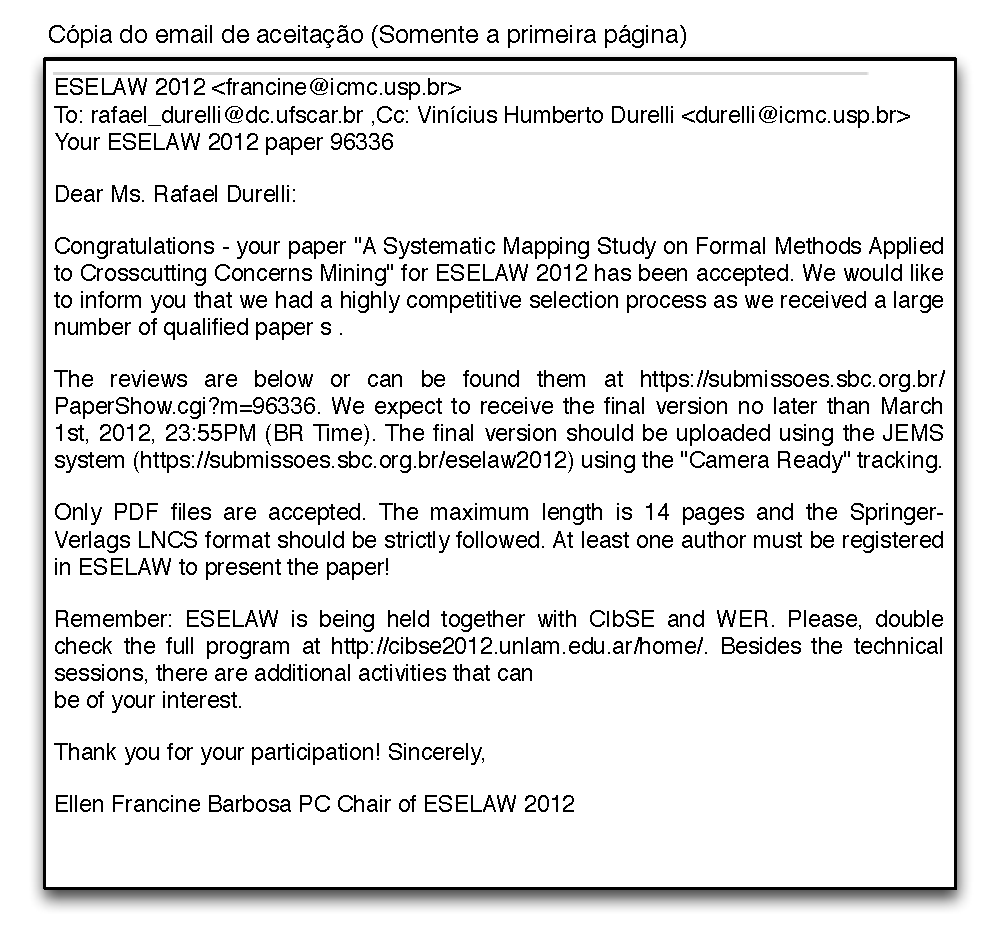
\includegraphics{apendices/comprovante_eselaw.pdf}}
 \label{fig:comprovante_vmil}
\end{figure}

\begin{itemize}
	\item Uma cópia do artigo é apresentado a seguir (a partir da próxima página).
\end{itemize}
\clearpage
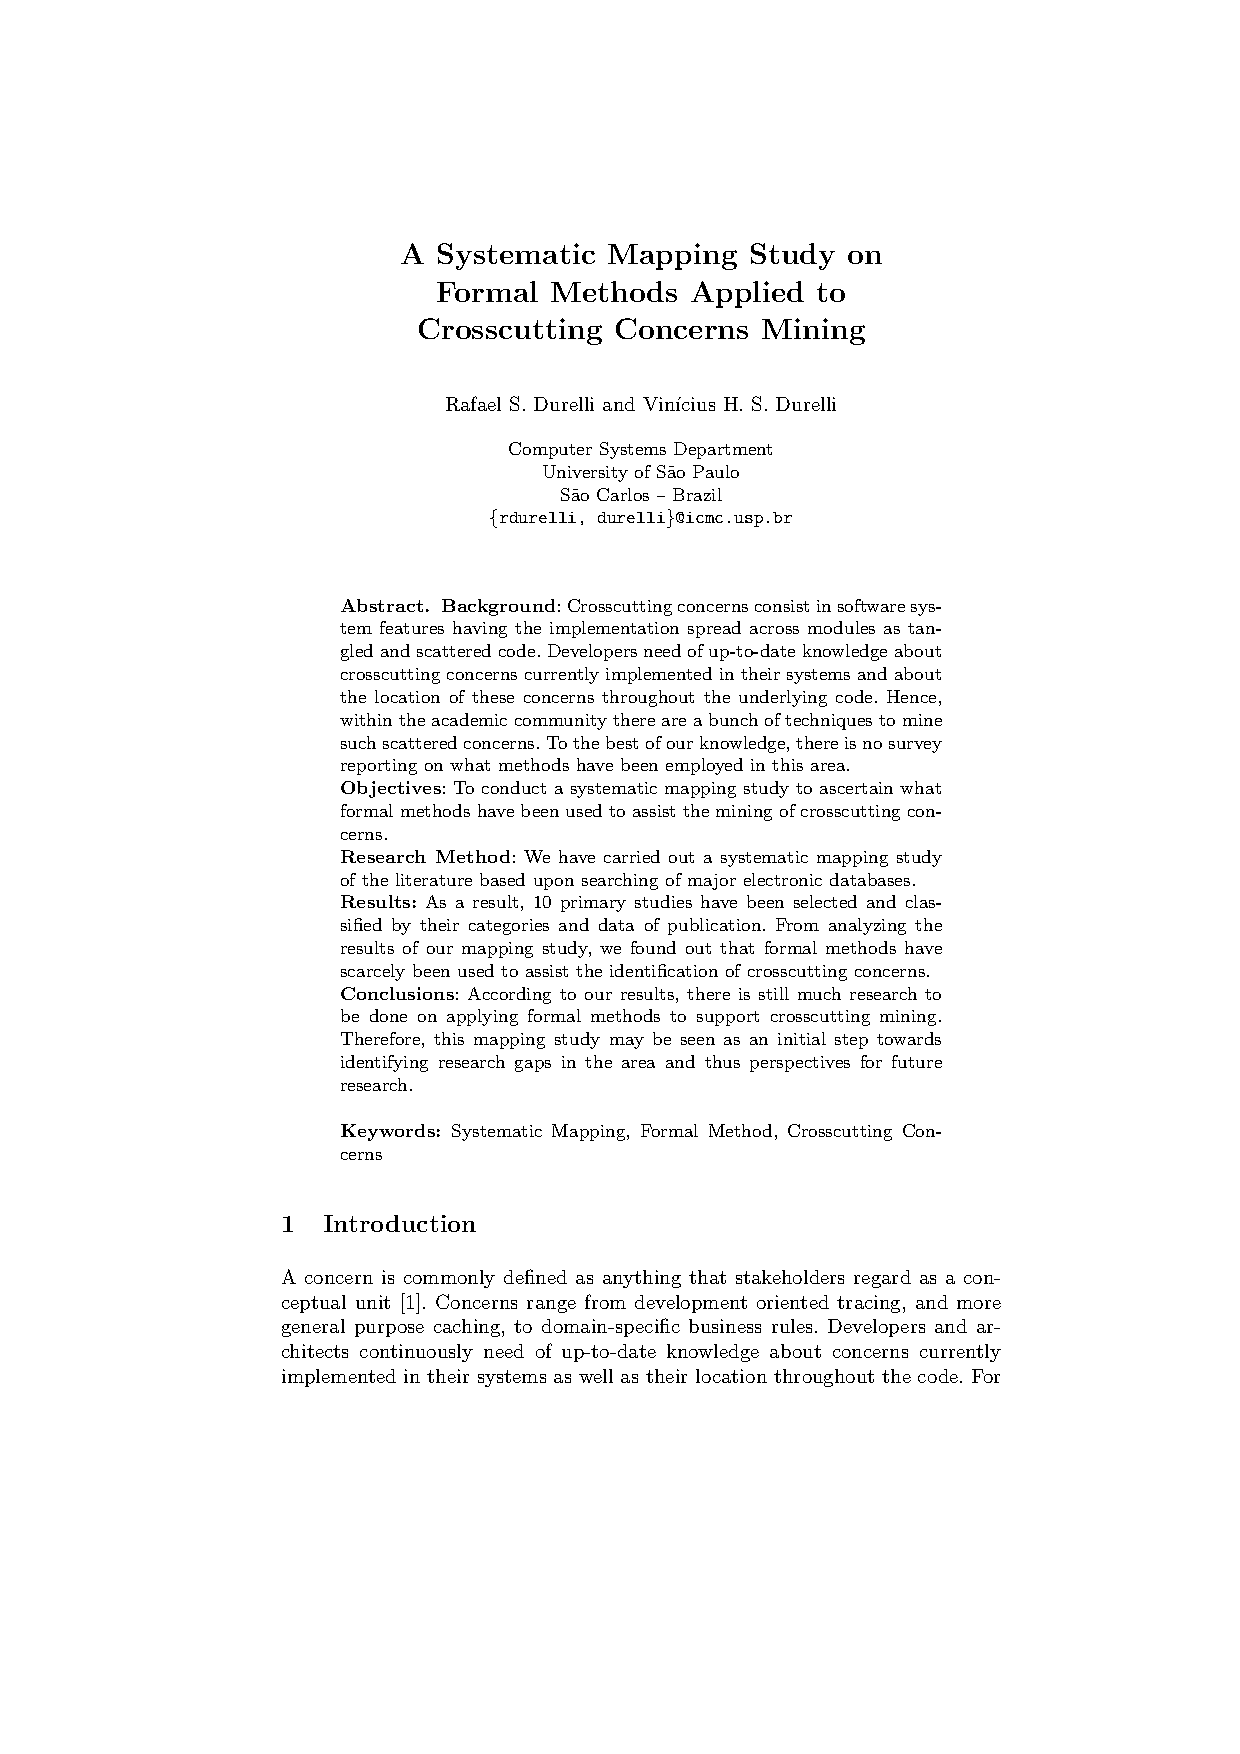
\includepdf[pages={-}]{apendices/mapeamento.pdf}

%--------anexo 2---------------------------------------------------------------

\subsection*{Anexo 2: Comprovante da publicação no \emph{Simpósio Brasileiro de Sistemas de Informação} (SBSI'12)} \label{anexo:comprovante_SBSI}

\addcontentsline{toc}{subsection}{Anexo 2: Comprovante da publicação no \emph{Simpósio Brasileiro de Sistemas de Informação} (SBSI'12)}

\begin{figure}[!h]
 \centering
 \scalebox{0.65}{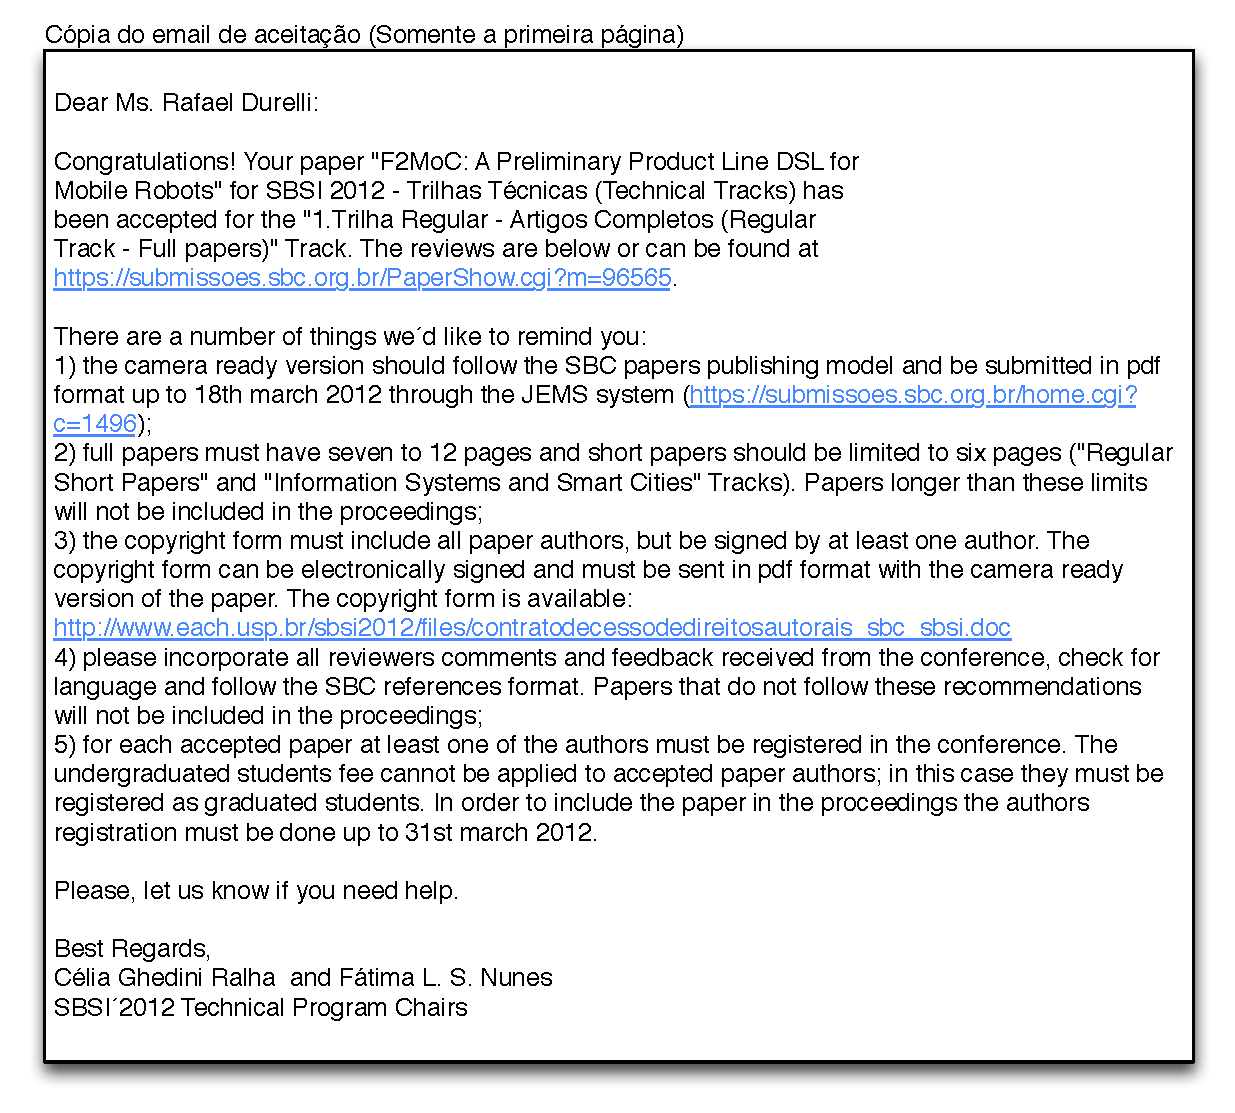
\includegraphics{apendices/comprovante_SBSI.pdf}}
 \label{fig:comprovante_vmil}
\end{figure}

\begin{itemize}
	\item Uma cópia do artigo é apresentado a seguir (a partir da próxima página).
\end{itemize}
\clearpage
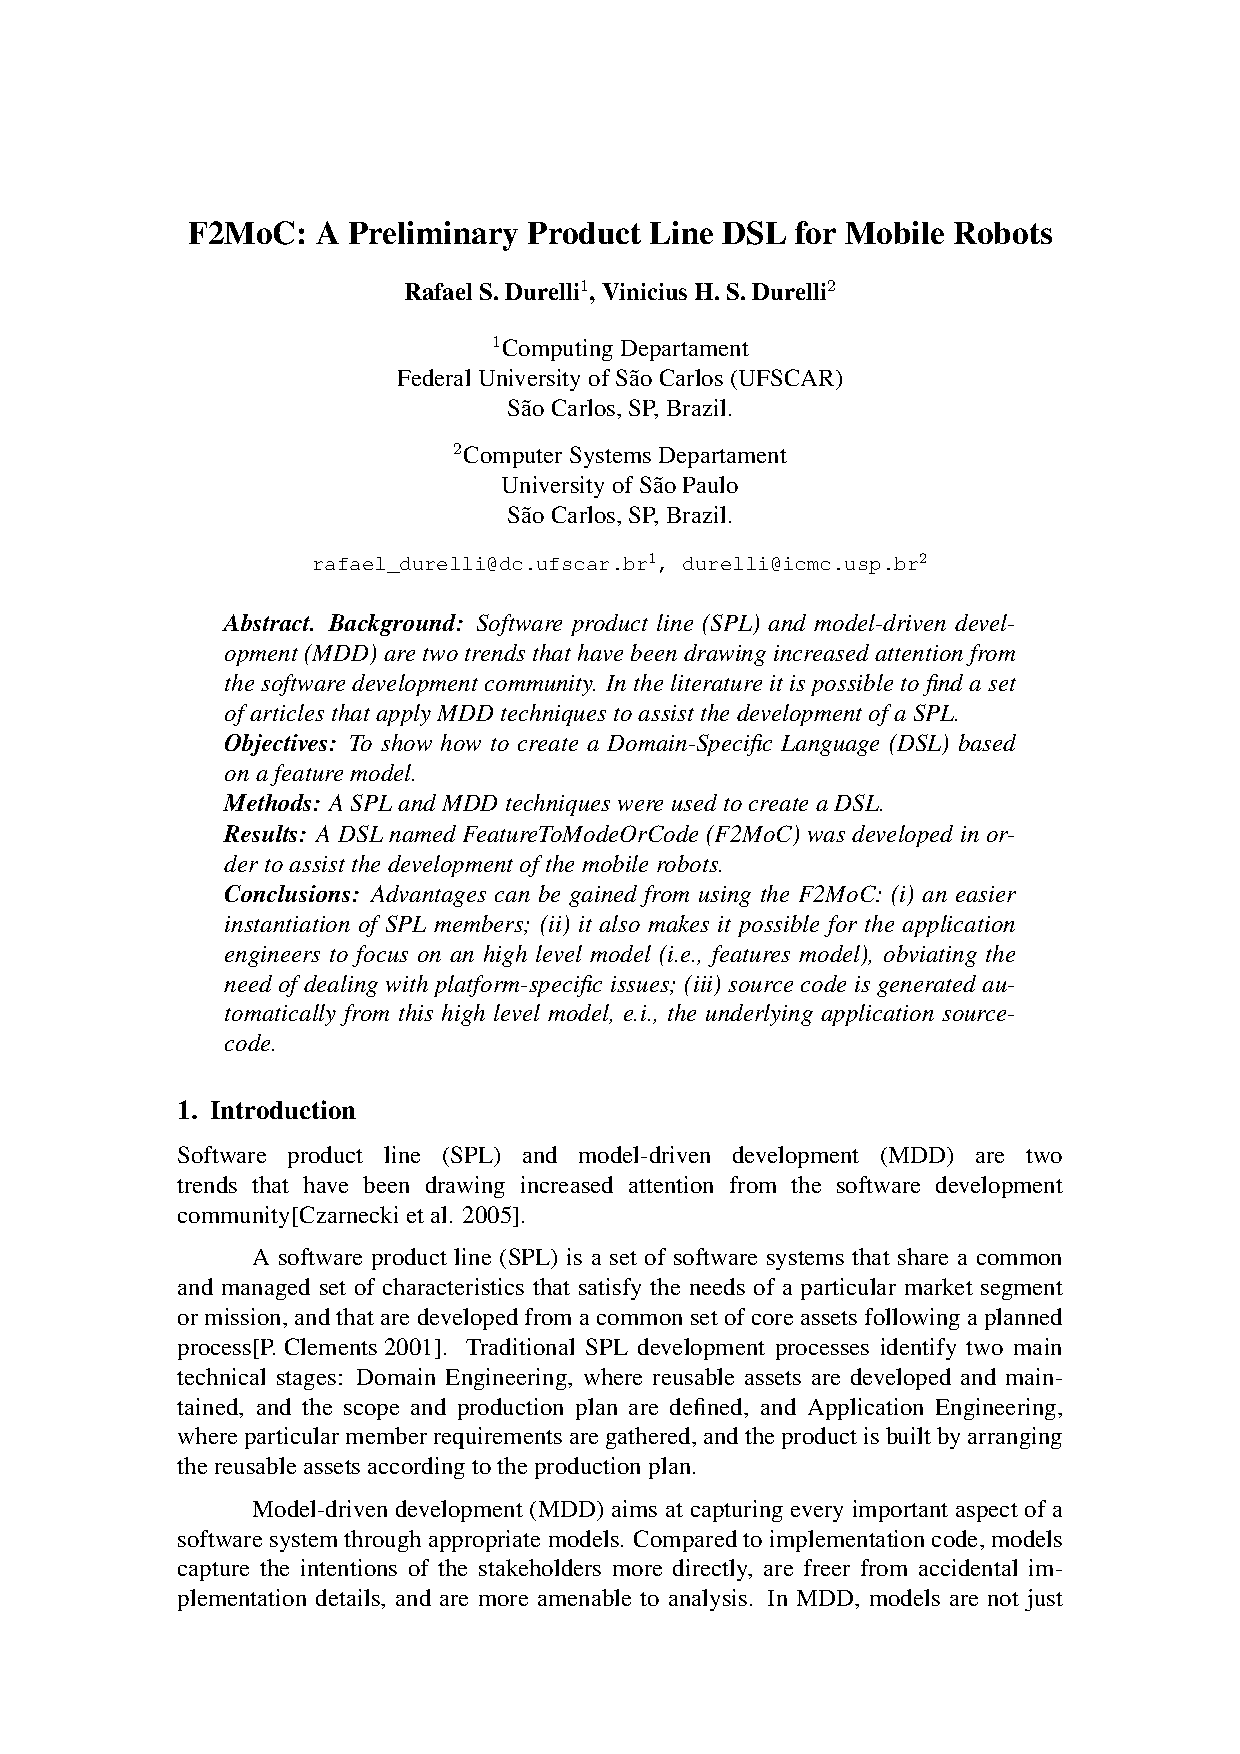
\includepdf[pages={-}]{apendices/SBSI.pdf}

%--------anexo 3---------------------------------------------------------------

\subsection*{Anexo 3: Comprovante da publicação no \emph{Simpósio Brasileiro de Engenharia de Software} (SBES'12)} \label{anexo:comprovante_SBES}

\addcontentsline{toc}{subsection}{Anexo 3: Comprovante da publicação no \emph{Simpósio Brasileiro de Engenharia de Software} (SBES'12)}

\begin{figure}[!h]
 \centering
 \scalebox{0.65}{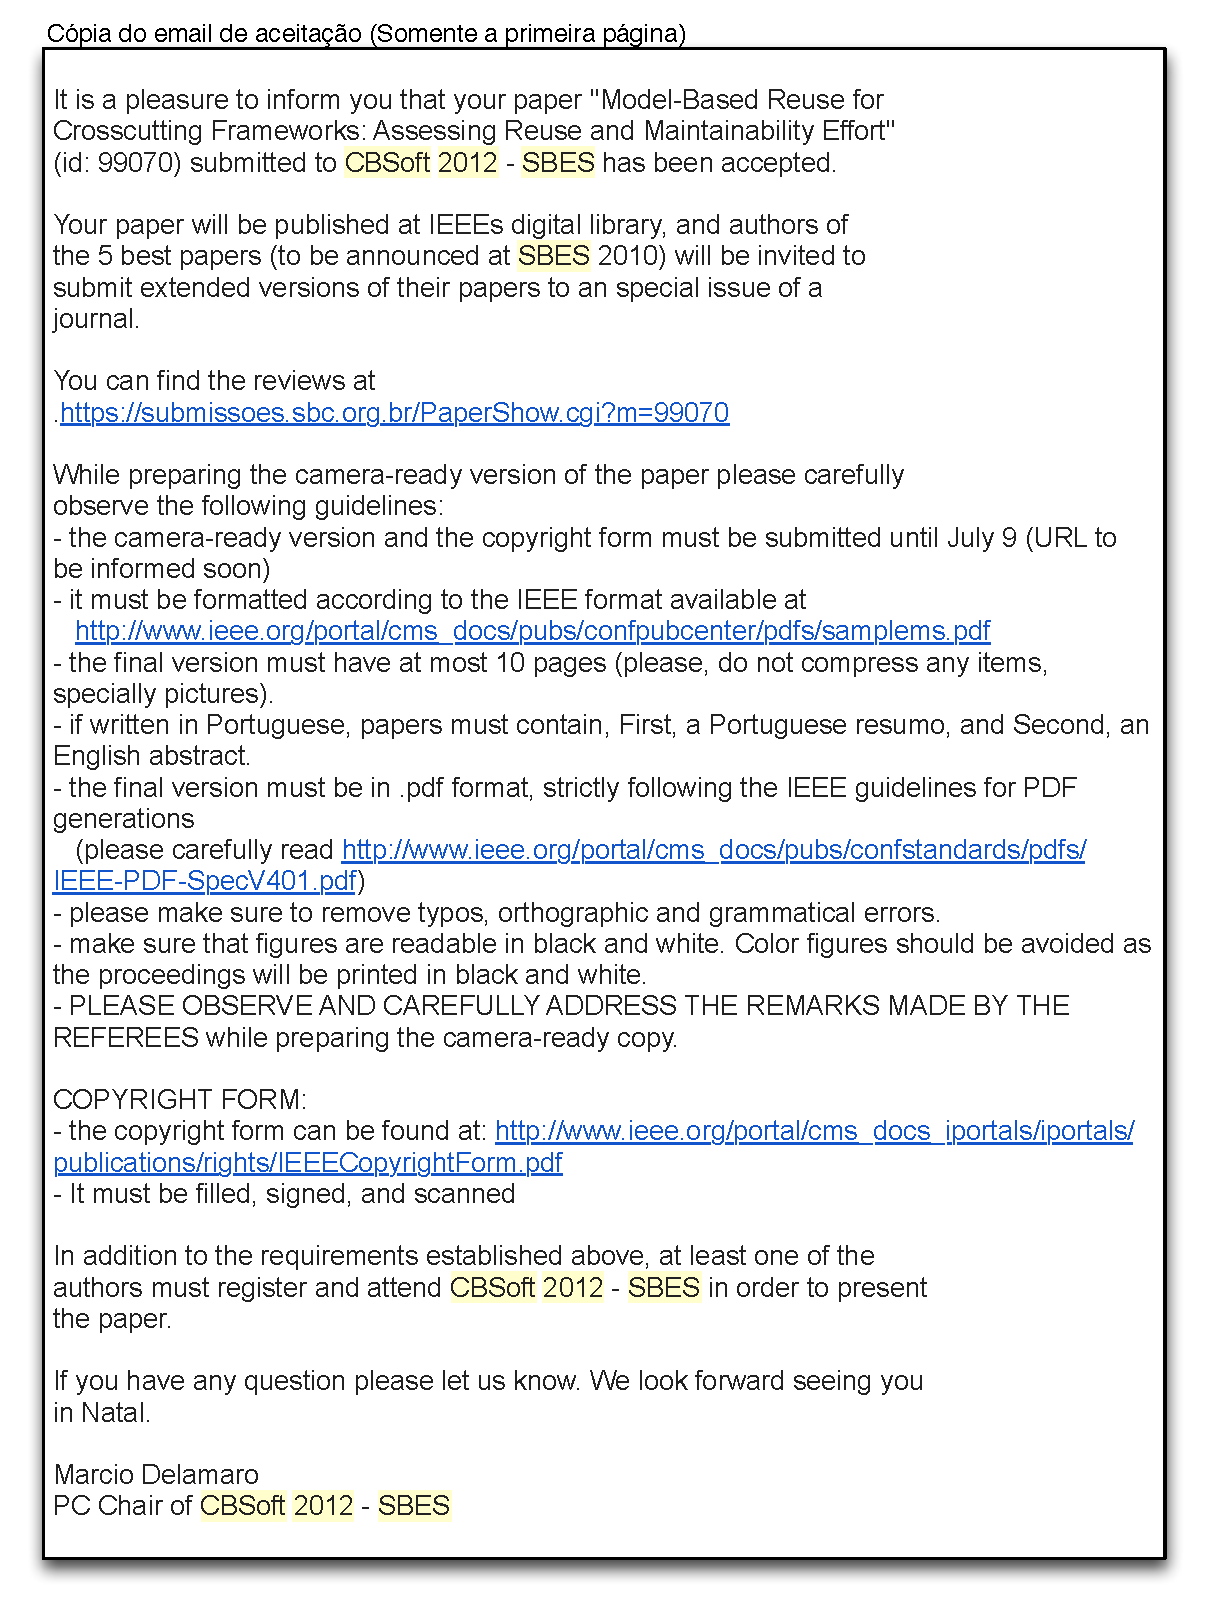
\includegraphics{apendices/comprovante_SBES.pdf}}
 \label{fig:comprovante_vmil}
\end{figure}

\begin{itemize}
	\item Uma cópia do artigo é apresentado a seguir (a partir da próxima página).
\end{itemize}
\clearpage
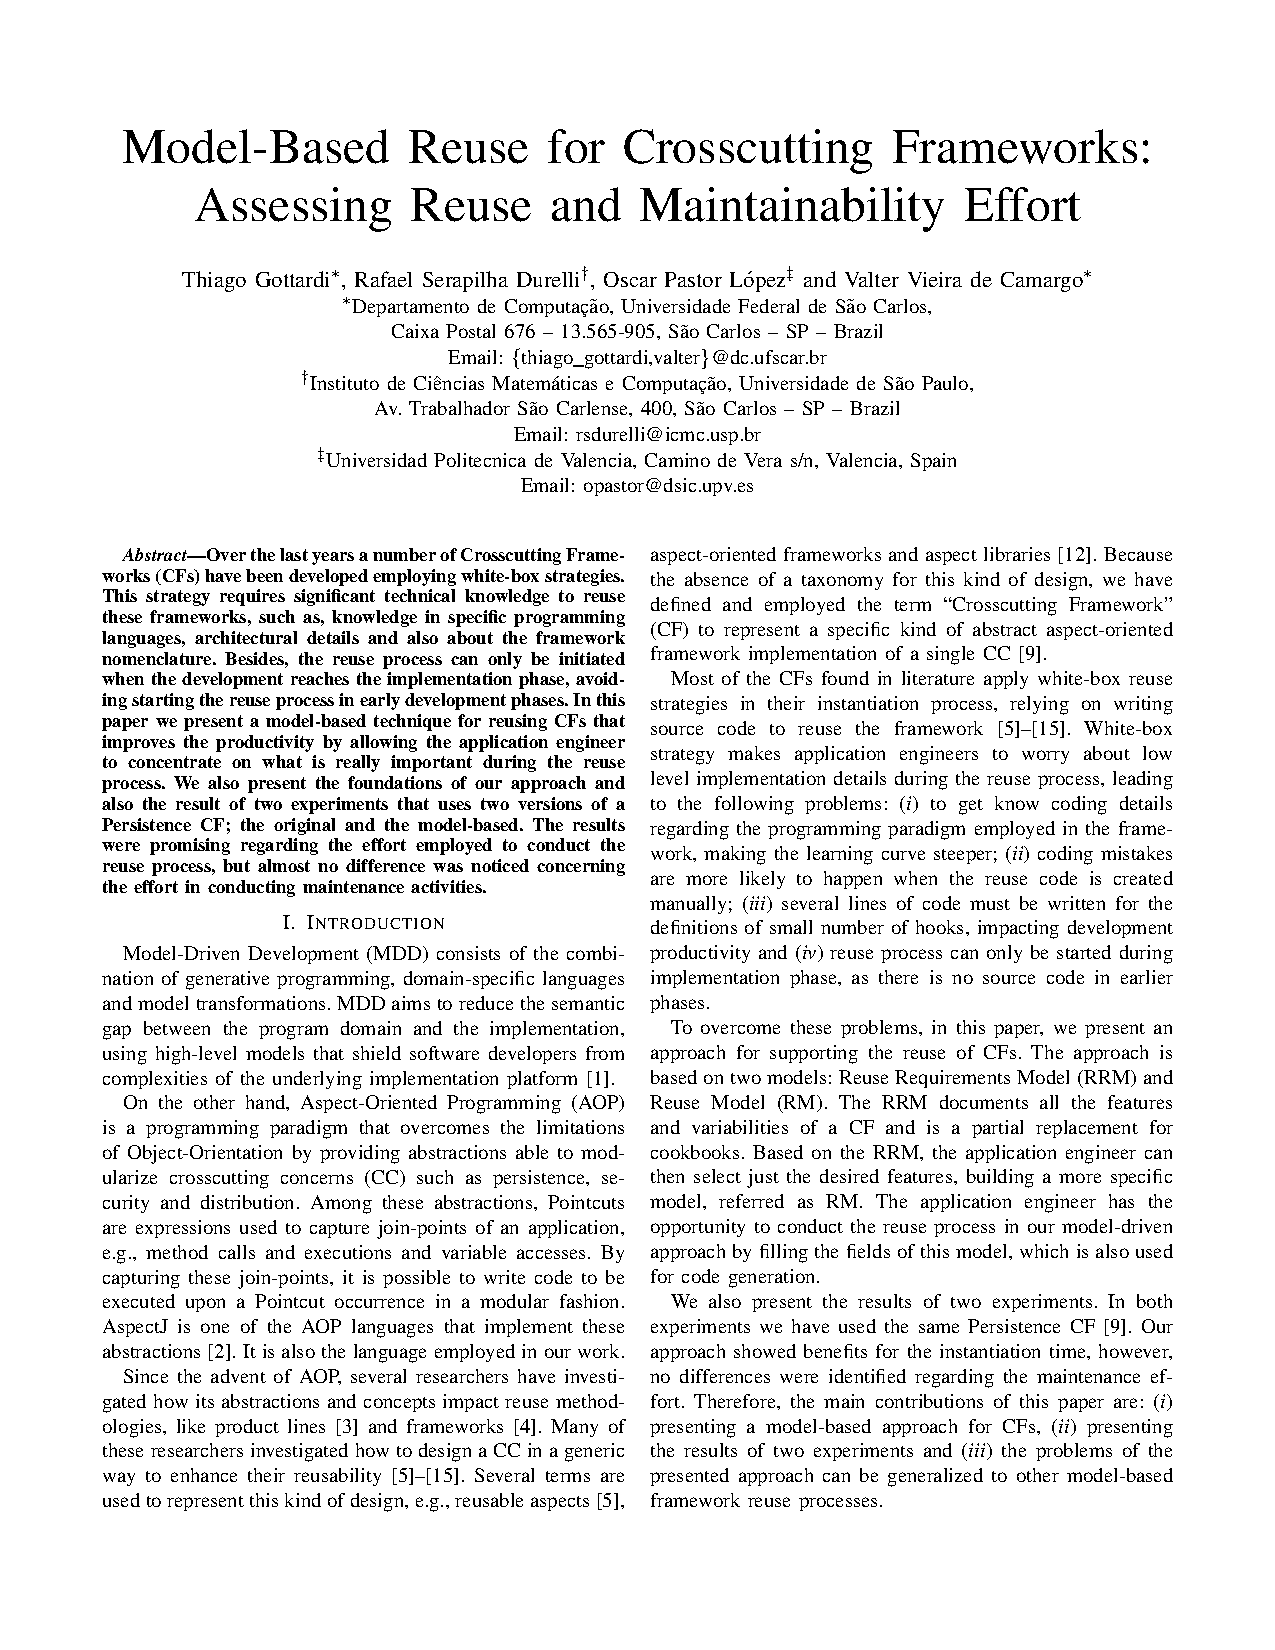
\includepdf[pages={-}]{apendices/sbes2012.pdf}

%--------anexo 4---------------------------------------------------------------

\subsection*{Anexo 4: Comprovante da publicação no \emph{Simpósio Brasileiro de Engenharia de Software - Sessão de Ferramentas} (SBES-Tools'12)} \label{anexo:comprovante_SBES}

\addcontentsline{toc}{subsection}{Anexo 4: Comprovante da publicação no \emph{Simpósio Brasileiro de Engenharia de Software - Sessão de Ferramentas} (SBES-Tools'12)}

\begin{figure}[!h]
 \centering
 \scalebox{0.65}{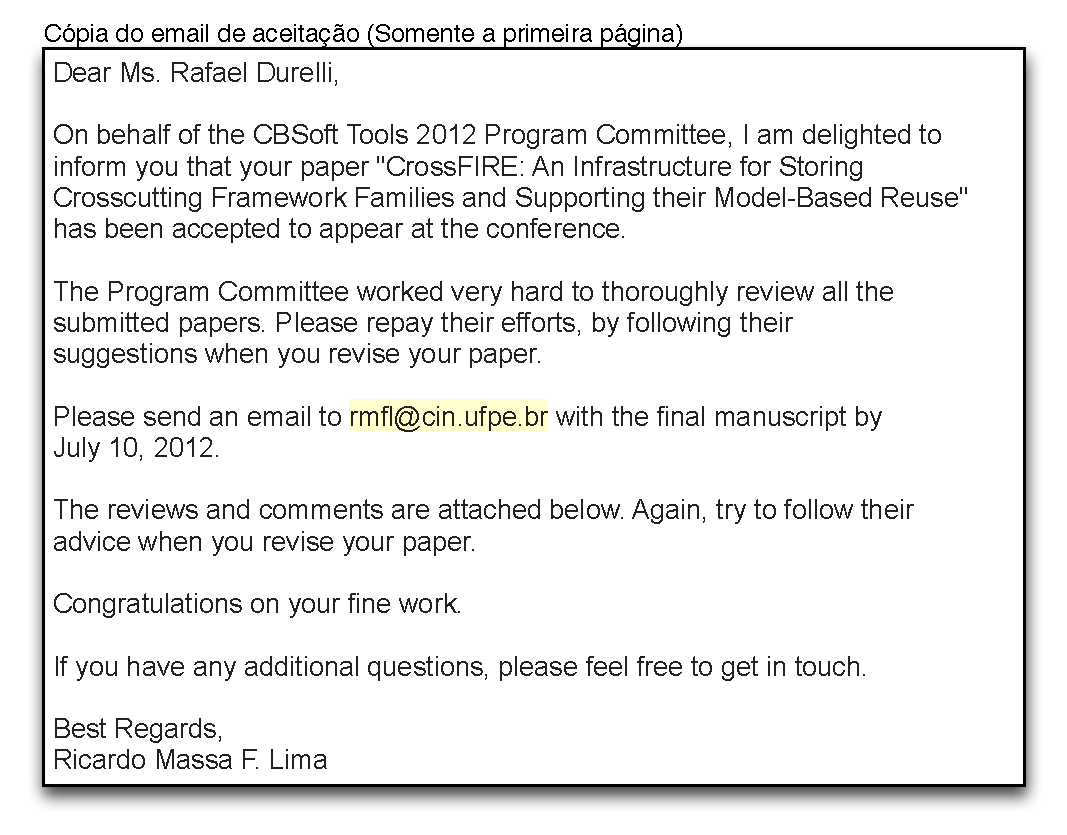
\includegraphics{apendices/comprovante_tools.pdf}}
 \label{fig:comprovante_vmil}
\end{figure}

\begin{itemize}
	\item Uma cópia do artigo é apresentado a seguir (a partir da próxima página).
\end{itemize}
\clearpage
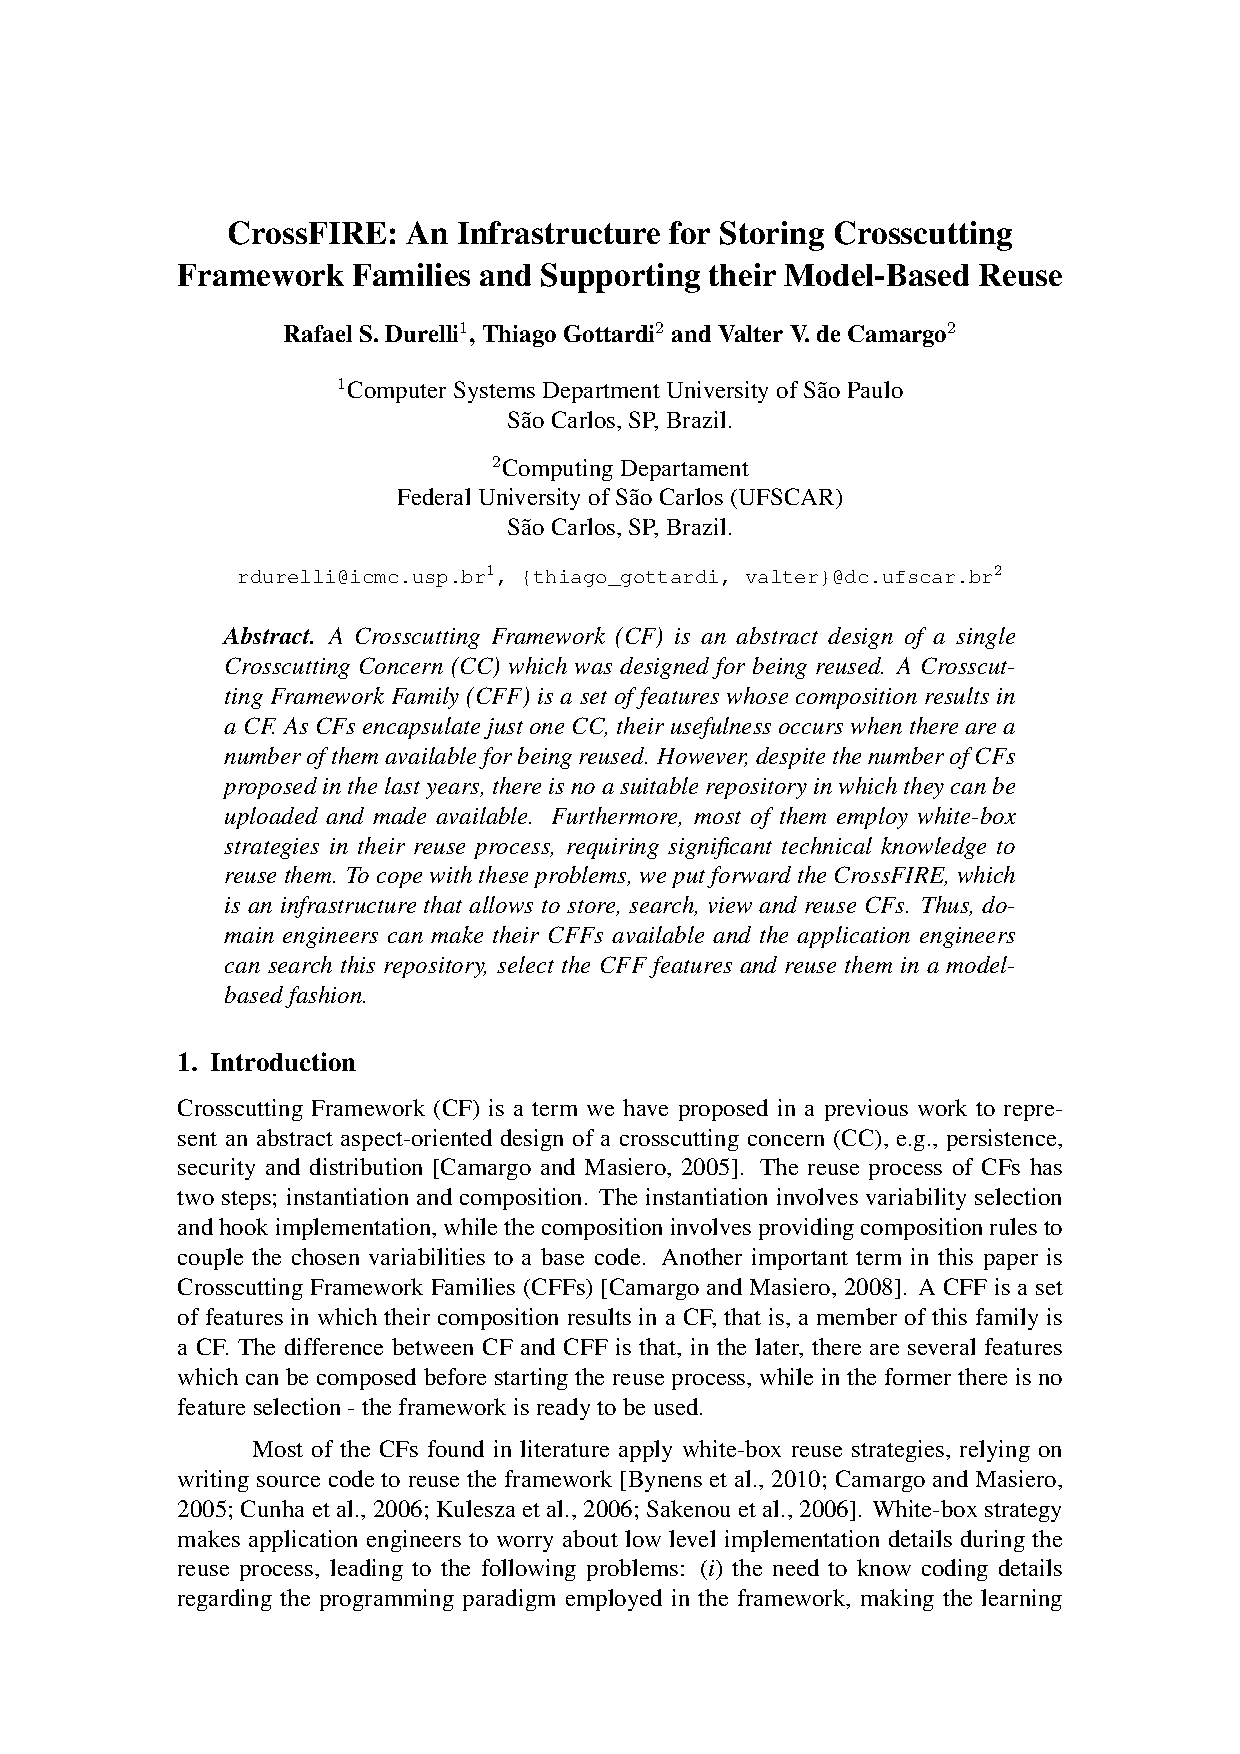
\includepdf[pages={-}]{apendices/SBESFerramenta.pdf}

%--------anexo 5---------------------------------------------------------------

\subsection*{Anexo 5: Comprovante da publicação no \emph{ACM SAC 2013} (SAC'13)} \label{anexo:comprovante_SBES}

\addcontentsline{toc}{subsection}{Anexo 5: Comprovante da publicação no \emph{ACM SAC 2013} (SAC'13)}

\begin{figure}[!h]
 \centering
 \scalebox{0.65}{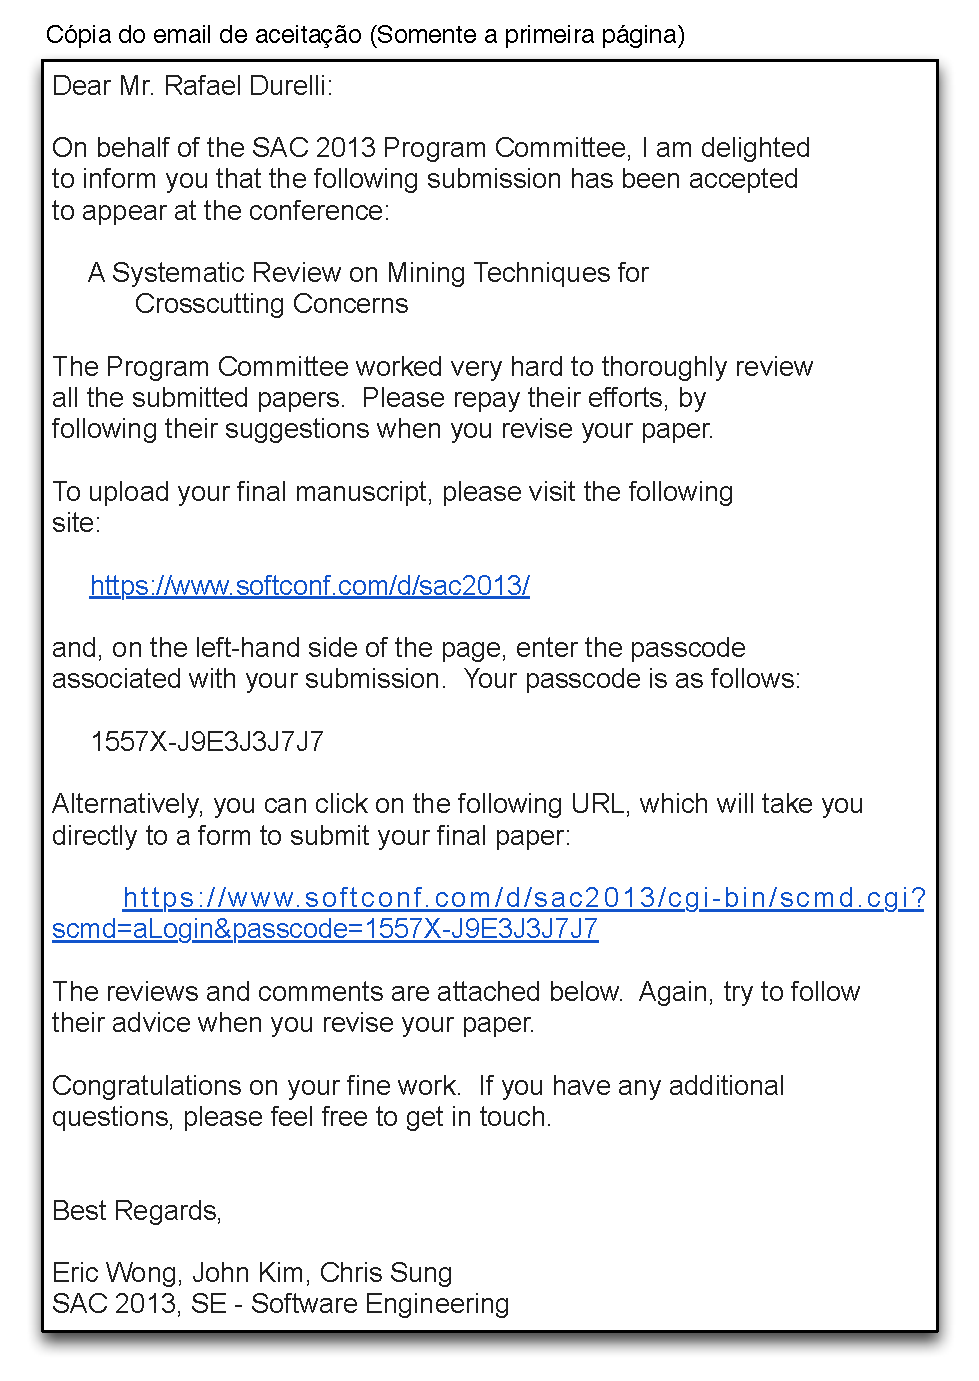
\includegraphics{apendices/comprovante_acmsac.pdf}}
 \label{fig:comprovante_vmil}
\end{figure}

\begin{itemize}
	\item Uma cópia do artigo é apresentado a seguir (a partir da próxima página).
\end{itemize}
\clearpage
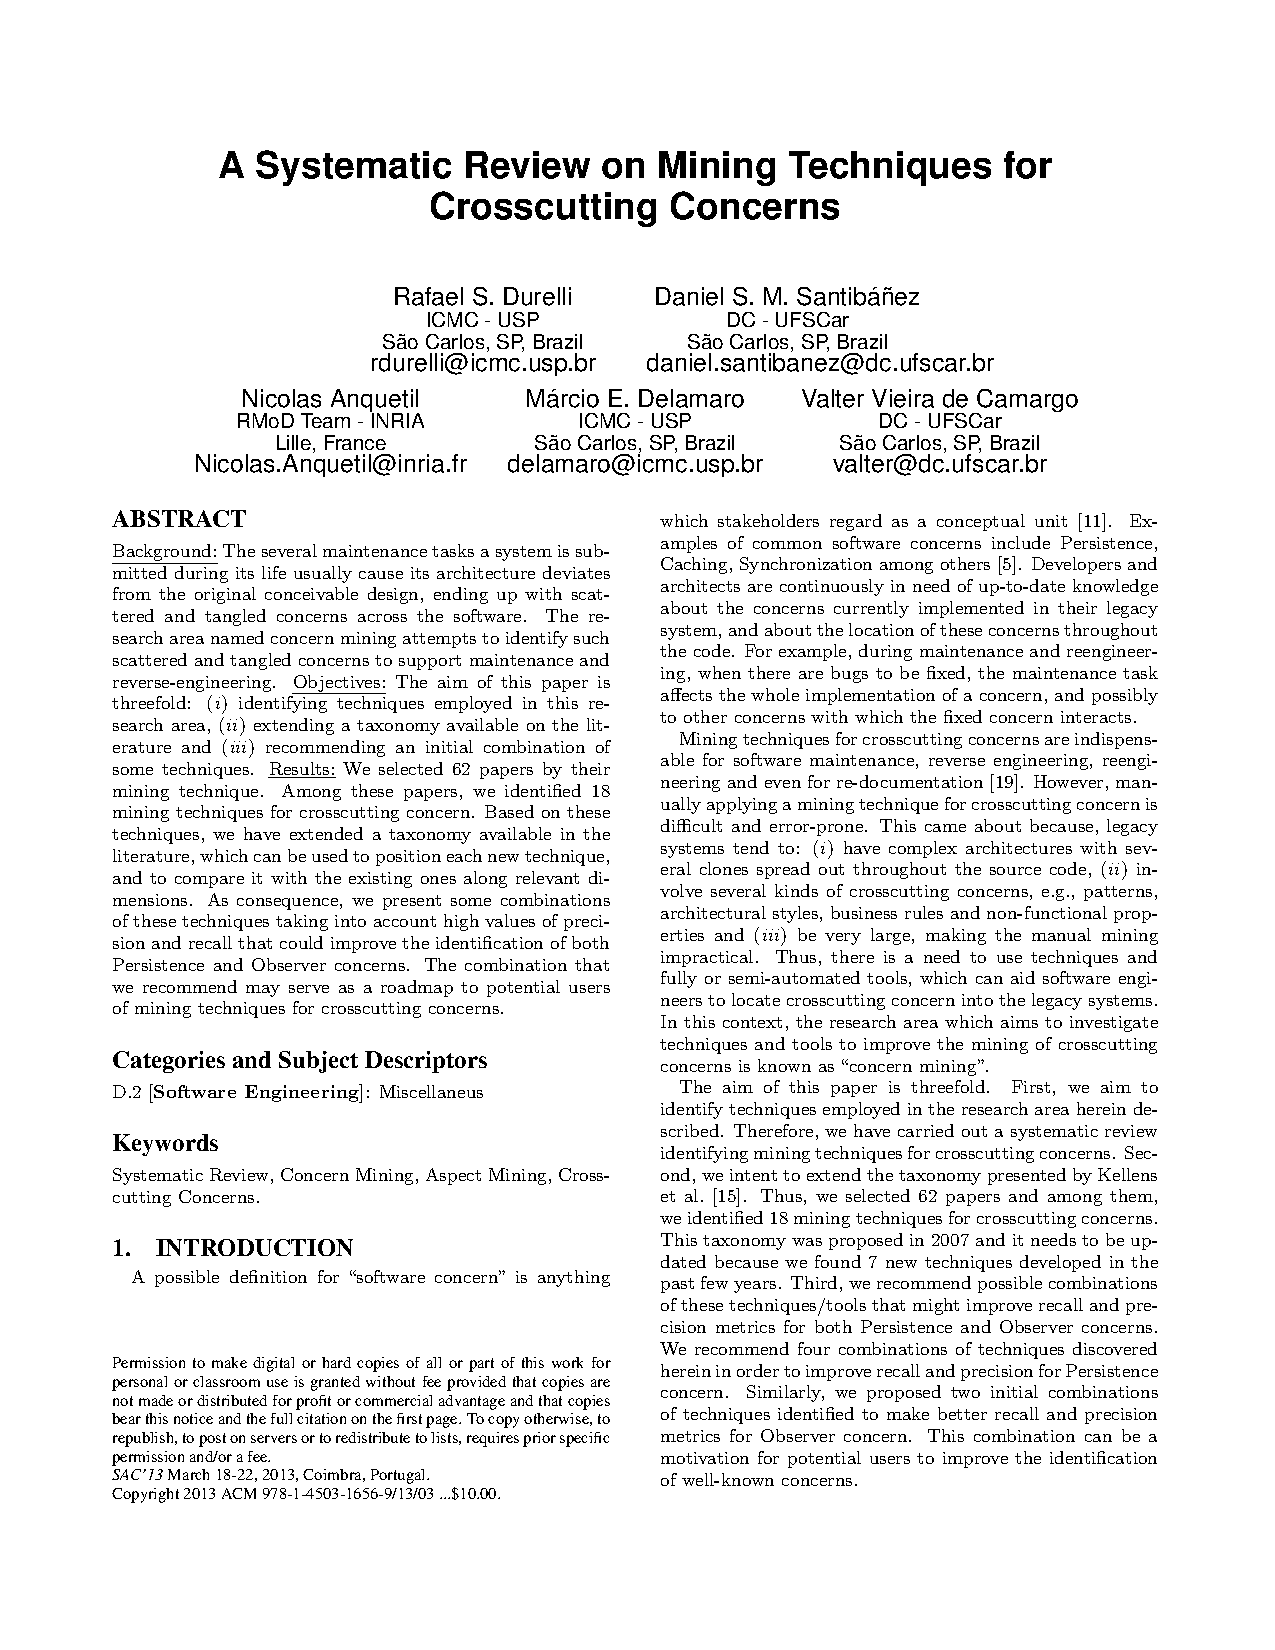
\includepdf[pages={-}]{apendices/acmSac2013.pdf}

%--------anexo 6---------------------------------------------------------------

\subsection*{Anexo 6: Comprovante da publicação no \emph{Latin-American Workshop on Aspect-Oriented Software Development 2012} (LA-WASP'12)} \label{anexo:comprovante_SBES}

\addcontentsline{toc}{subsection}{Anexo 6: Comprovante da publicação no \emph{Latin-American Workshop on Aspect-Oriented Software Development 2012} (LA-WASP'12)}

\begin{figure}[!h]
 \centering
 \scalebox{0.65}{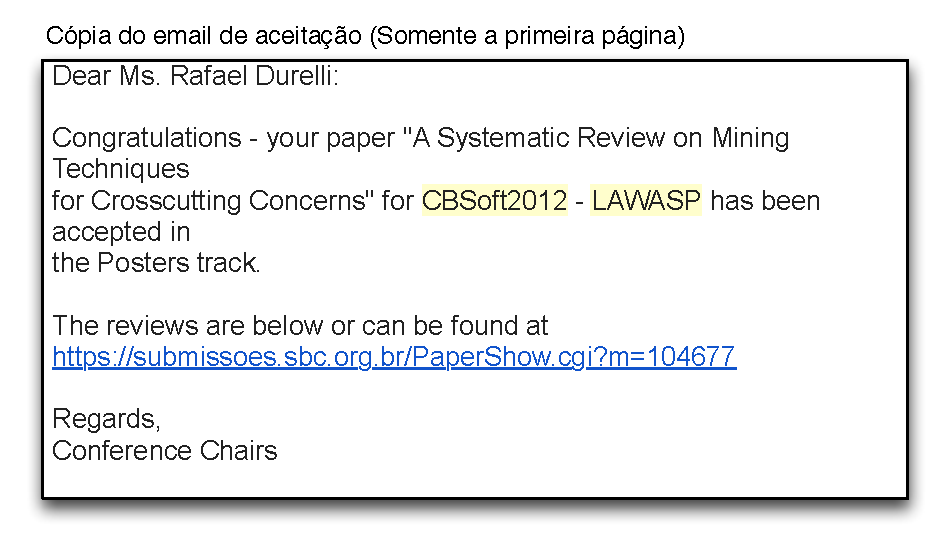
\includegraphics{apendices/comprovante_lawasp.pdf}}
 \label{fig:comprovante_vmil}
\end{figure}

\begin{itemize}
	\item Uma cópia do artigo é apresentado a seguir (a partir da próxima página).
\end{itemize}
\clearpage
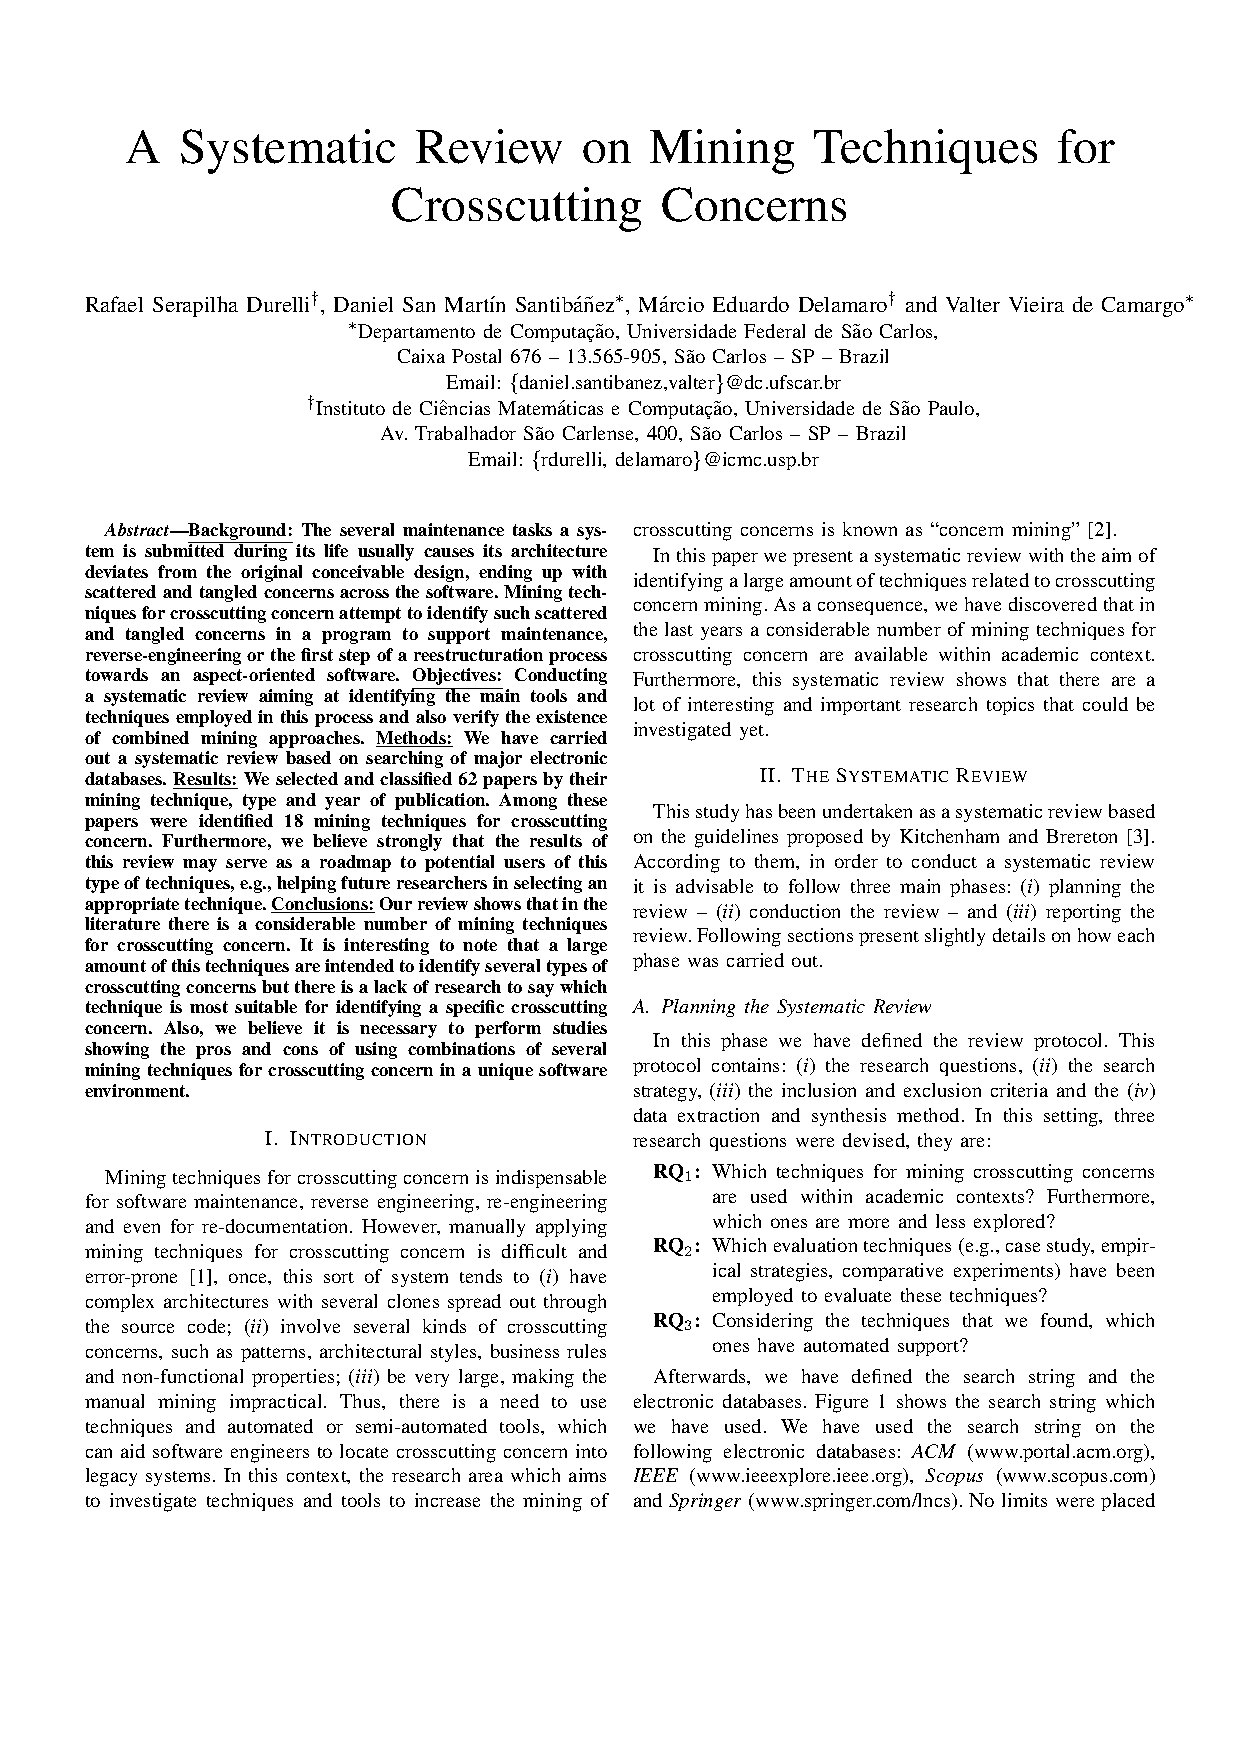
\includepdf[pages={-}]{apendices/laWasp2012Poster.pdf}


\end{document}
